% Pengaturan ukuran teks dan bentuk halaman dua sisi
\documentclass[10pt,twoside]{report}

% Pengaturan ukuran halaman dan margin
\usepackage[a5paper,top=25mm,left=25mm,right=20mm,bottom=25mm]{geometry}

% Pengaturan ukuran spasi
\usepackage[singlespacing]{setspace}

% Judul dokumen
\title{Buku Laporan Kerja Praktik ITS}
\author{Musk, Elon Reeve \and Kjellberg, Felix Arvid Ulf}

% Pengaturan format bahasa
\usepackage[indonesian]{babel}

% Pengaturan detail pada file PDF
\usepackage[pdfauthor={\@author},bookmarksnumbered,pdfborder={0 0 0}]{hyperref}

% Pengaturan jenis karakter
\usepackage[utf8]{inputenc}

% Pengaturan ukuran indentasi paragraf
\setlength{\parindent}{2em}

% Pengaturan ukuran spasi paragraf
\setlength{\parskip}{0.5ex}

% Package lainnya
\usepackage{etoolbox} % Mengubah fungsi default
\usepackage{enumitem} % Pembuatan list
\usepackage{lipsum} % Pembuatan template kalimat
\usepackage{graphicx} % Input gambar
\usepackage{longtable} % Pembuatan tabel
\usepackage[table,xcdraw]{xcolor} % Pewarnaan tabel
\usepackage[numbers]{natbib} % Kutipan artikel
\usepackage{eso-pic} % Pembuatan background
\usepackage{changepage} % Pembuatan teks kolom
\usepackage{wrapfig} % Wrapping gambar

% Definisi untuk "Hati ini sengaja dikosongkan"
\def\kosong{
  \vspace*{\fill}
  \begin{center}\textit{Halaman ini sengaja dikosongkan}\end{center}
  \vfill
}
\patchcmd{\cleardoublepage}{\hbox{}}{\kosong}{}{}

% Pengaturan penomoran halaman
\usepackage{fancyhdr}
\fancyhf{}
\renewcommand{\headrulewidth}{0pt}
\pagestyle{fancy}
\fancyfoot[CE,CO]{\thepage}
\patchcmd{\chapter}{plain}{fancy}{}{}
\patchcmd{\chapter}{empty}{plain}{}{}

% Pengaturan format judul bab
\usepackage{titlesec}
\titleformat{\chapter}[display]{\bfseries\Large}{BAB \centering\Roman{chapter}}{0ex}{\vspace{0ex}\centering}[\vspace{2ex}]
\titleformat{\section}{\bfseries\large}{\MakeUppercase{\thesection}}{1ex}{}
\titleformat{\subsection}{\bfseries\large}{\MakeUppercase{\thesubsection}}{1ex}{}
\titleformat{\subsubsection}{\bfseries\large}{\MakeUppercase{\thesubsubsection}}{1ex}{}
\titlespacing{\chapter}{0ex}{0ex}{2ex}
\titlespacing{\section}{0ex}{2ex}{1ex}
\titlespacing{\subsection}{0ex}{1ex}{0.5ex}
\titlespacing{\subsubsection}{0ex}{1ex}{0.5ex}

% Pengaturan persamaan
\newenvironment{conditions}
{\par\vspace{\abovedisplayskip}\noindent
  \tabularx{\columnwidth}{>{$}l<{$} @{${}={}$} >{\raggedright\arraybackslash}X}}
{\endtabularx\par\vspace{\belowdisplayskip}}

% Pengaturan format baris program
\usepackage{listings}
\definecolor{comment}{RGB}{0,128,0}
\definecolor{string}{RGB}{255,0,0}
\definecolor{keyword}{RGB}{0,0,255}
\lstdefinestyle{codestyle}{
  commentstyle=\color{comment},
  stringstyle=\color{string},
  keywordstyle=\color{keyword},
  basicstyle=\footnotesize\ttfamily,
  numbers=left,
  numberstyle=\tiny,
  numbersep=5pt,
  frame=lines,
  breaklines=true,
  prebreak=\raisebox{0ex}[0ex][0ex]{\ensuremath{\hookleftarrow}},
  showstringspaces=false,
  upquote=true,
  tabsize=2,
}
\lstset{style=codestyle}

% Isi keseluruhan dokumen
\begin{document}

  % Nomor halaman pembuka dimulai dari sini
  \pagenumbering{roman}

  % Sampul luar
  % \AddToShipoutPictureBG*{
  \AtPageLowerLeft{
    % Ubah nilai berikut jika posisi horizontal background tidak sesuai
    \hspace{-3.5mm}

    % Ubah nilai berikut jika posisi vertikal background tidak sesuai
    \raisebox{0mm}{
      
\includegraphics[width=\paperwidth,height=\paperheight]{sampul/sampul-luar.png}
    }
  }
}

% Menyembunyikan nomor halaman
\thispagestyle{empty}

% Pengaturan margin untuk menyesuaikan konten sampul
\newgeometry{top=70mm,left=25mm,right=20mm,bottom=25mm}

\begin{flushleft}

  % Pengaturan jenis dan warna teks yang digunakan
  \sffamily\color{white}

  % Ubah penomoran buku berikut sesuai dengan yang ditentukan oleh departemen
  \noindent\textbf{KERJA PRAKTIK - EC184601}
  \vspace{4ex}

  % Ubah kalimat berikut sesuai dengan nama perusahaan tempat kerja praktik
  \noindent{\large \textbf{DEPARTEMEN TEKNIK KOMPUTER}} \\
  % Ubah tanggal berikut sesuai dengan waktu berlangsungnya kerja praktik
  \textbf{(03 Agustus 2021 s/d 03 September 2021)}
  \vspace{6ex}

  % Ubah kalimat berikut sesuai dengan judul topik kerja praktik
  \noindent{\large \textbf{INSTALASI FACE RECOGNITION SYSTEM DI PERKANTORAN}}
  \vspace{6ex}

  \begin{adjustwidth}{-2mm}{}
    \begin{tabular}{lcp{0.7\linewidth}}
      % Ubah kalimat-kalimat berikut sesuai dengan nama dan NRP mahasiswa pertama
      \textbf{Awang Ivananto Adi} & & \textbf{NRP 0721 18 4000 0007} \\
      % Ubah kalimat-kalimat berikut sesuai dengan nama dan NRP mahasiswa kedua
      \textbf{Annida M F} & & \textbf{NRP 0721 18 4000 0030} \\
      % Ubah kalimat-kalimat berikut sesuai dengan nama dan NRP mahasiswa kedua
      \textbf{Suryo Adiguna} & & \textbf{NRP 0721 18 4000 0052} \\
    \end{tabular}
  \end{adjustwidth}
  \vspace{4ex}

  \noindent\textbf{Dosen Pembimbing} \\
  % Ubah kalimat berikut sesuai dengan nama dosen pembimbing
  \textbf{Dr.Supeno Mardi Susiki Nugroho ST., M.T.}
  \vspace{10ex}

  % Ubah kalimat berikut sesuai dengan nama departemen
  \noindent\textbf{DEPARTEMEN TEKNIK KOMPUTER} \\
  % Ubah kalimat berikut sesuai dengan nama fakultas
  \textbf{Fakultas Teknologi Elektro dan Informatika Cerdas} \\
  \textbf{Institut Teknologi Sepuluh Nopember} \\
  % Ubah kalimat berikut sesuai dengan tempat dan tahun pembuatan buku
  \textbf{Surabaya 2021}

\end{flushleft}

\restoregeometry

  % \cleardoublepage

  % Sampul dalam
  \AddToShipoutPictureBG*{
  \AtPageLowerLeft{
    % Ubah nilai berikut jika posisi horizontal background tidak sesuai
    \hspace{-3.5mm}

    % Ubah nilai berikut jika posisi vertikal background tidak sesuai
    \raisebox{0mm}{
      
\includegraphics[width=\paperwidth,height=\paperheight]{sampul/sampul-dalam.png}
    }
  }
}

% Pengaturan margin untuk menyesuaikan konten sampul
\newgeometry{top=70mm,left=25mm,right=20mm,bottom=25mm}

\begin{flushleft}

  % Pengaturan jenis teks yang digunakan
  \sffamily

  % Ubah penomoran buku berikut sesuai dengan yang ditentukan oleh departemen
  \noindent\textbf{KERJA PRAKTIK - TD123456}
  \vspace{4ex}

  % Ubah kalimat berikut sesuai dengan nama perusahaan tempat kerja praktik
  \noindent{\large \textbf{PT. NATIONAL AERONAUTICS AND SPACE ADMINISTRATION}} \\
  % Ubah tanggal berikut sesuai dengan waktu berlangsungnya kerja praktik
  \textbf{(03 Desember 2020 s/d 03 Januari 2021)}
  \vspace{6ex}

  % Ubah kalimat berikut sesuai dengan judul topik kerja praktik
  \noindent{\large \textbf{PEMBUATAN ROKET LUAR ANGKASA ANTI GRAVITASI UNTUK PT. NASA}}
  \vspace{6ex}

  \begin{adjustwidth}{-2mm}{}
    \begin{tabular}{lcp{0.7\linewidth}}
      % Ubah kalimat-kalimat berikut sesuai dengan nama dan NRP mahasiswa pertama
      \textbf{Elon Reeve Musk} & & \textbf{NRP 0123 20 4000 0001} \\
      % Ubah kalimat-kalimat berikut sesuai dengan nama dan NRP mahasiswa kedua
      \textbf{Felix Arvid Ulf Kjellberg} & & \textbf{NRP 0123 20 4000 0002} \\
    \end{tabular}
  \end{adjustwidth}
  \vspace{4ex}

  \noindent
  \textbf{Dosen Pembimbing} \\
  % Ubah kalimat berikut sesuai dengan nama dosen pembimbing
  \textbf{Nikola Tesla, S.T., M.T.}
  \vspace{10ex}

  % Ubah kalimat berikut sesuai dengan nama departemen
  \noindent\textbf{DEPARTEMEN TEKNIK DIRGANTARA} \\
  % Ubah kalimat berikut sesuai dengan nama fakultas
  \textbf{Fakultas Teknologi Dirgantara} \\
  \textbf{Institut Teknologi Sepuluh Nopember} \\
  % Ubah kalimat berikut sesuai dengan tempat dan tahun pembuatan buku
  \textbf{Surabaya 2021}

\end{flushleft}

\restoregeometry

  \cleardoublepage

  % Lembar pengesahaan untuk departemen
  \begin{center}
  {\Large \textbf{LEMBAR PENGESAHAN}}
  \vspace{6ex}

  \addcontentsline{toc}{chapter}{LEMBAR PENGESAHAN (DEPARTEMEN)}

  % Ubah kalimat berikut sesuai dengan judul topik kerja praktik
  {\large \textbf{PEMBUATAN ROKET LUAR ANGKASA ANTI GRAVITASI UNTUK PT. NASA}}
  \vspace{6ex}

  % Ubah kalimat berikut sesuai dengan kalimat pengesahan yang ditentukan oleh departemen
  Laporan Kerja Praktik ini disusun untuk \lipsum[1][1]
  \vspace{2ex}

  % Ubah kalimat-kalimat berikut sesuai dengan tempat dan tanggal pengesahan
  Tempat Pengesahan di: Surabaya \\
  Tanggal: 03 Februari 2021
  \vspace{8ex}

  Menyetujui, \\
  Dosen Pembimbing,
  \vspace{12ex}

  % Ubah kalimat-kalimat berikut sesuai dengan nama dan NIP dosen pembimbing
  \textbf{\underline{Nikola Tesla, S.T., M.T.}} \\
  NIP. 18560710 194301 1 001
  \vspace{8ex}

  Mengetahui, \\
  % Ubah kalimat berikut sesuai dengan jabatan kepala departemen
  Kepala Departemen Teknik Dirgantara FTD - ITS,
  \vspace{12ex}

  % Ubah kalimat-kalimat berikut sesuai dengan nama dan NIP kepala departemen
  \textbf{\underline{Dr. Leonardo Da Vinci, S.T., M.T.}} \\
  NIP 14520415 151905 1 001

\end{center}

  \cleardoublepage

  % Lembar pengesahan untuk perusahaan
  \begin{center}
  {\Large \textbf{LEMBAR PENGESAHAN}}
  \vspace{6ex}

  \addcontentsline{toc}{chapter}{LEMBAR PENGESAHAN (PERUSAHAAN)}

  % Ubah kalimat berikut sesuai dengan judul topik kerja praktik
  {\large \textbf{PEMBUATAN ROKET LUAR ANGKASA ANTI GRAVITASI UNTUK PT. NASA}}
  \vspace{6ex}

  % Ubah kalimat berikut sesuai dengan kalimat pengesahan yang ditentukan oleh departemen
  Laporan Kerja Praktik ini disusun untuk \lipsum[1][1]
  \vspace{2ex}

  % Ubah kalimat-kalimat berikut sesuai dengan tempat dan tanggal pengesahan
  Tempat Pengesahan di: Surabaya \\
  Tanggal: 03 Februari 2021
  \vspace{8ex}

  Mengetahui, \\
  Pembimbing Perusahaan
  \vspace{12ex}

  % Ubah kalimat berikut sesuai dengan nama pembimbing perusahaan
  \textbf{\underline{Yuri Gagarin, S.Si., M.Si.}}
  \vspace{8ex}

  Mengetahui, \\
  % Ubah kalimat berikut sesuai dengan jabatan kepala perusahaan
  Chief Executive Officer PT. NASA
  \vspace{12ex}

  % Ubah kalimat berikut sesuai dengan nama kepala perusahaan.
  \textbf{\underline{Dr. Galileo Galilei, S.Si., M.Si.}}

\end{center}

  \cleardoublepage

  % Kata pengantar
  \begin{center}
  \Large\textbf{KATA PENGANTAR}
\end{center}
\vspace{2ex}

\addcontentsline{toc}{chapter}{KATA PENGANTAR}

% Ubah paragraf-paragraf berikut sesuai dengan yang ingin diisi pada kata pengantar

Puji syukur kami ucapkan kepada Tuhan Yang Maha Esa karena atas petunjuk dan rahmatNya, penulis telah dapat menyeleasikan Kerja Praktik di Departemen Teknik Komputer, FTEIC, ITS yang dilaksanakan tanggal 3 Agustus 2021 sampai dengan 3 September 2021

Dalam penyelesaian Laporan Kerja Praktik ini, kami mengucapkan terima kasih kepada berbagai pihak yang telah membantu terselesaikannya laporan ini hingga akhir:

\begin{enumerate}[nolistsep]

  \item Bapak Dr. Supeno Mardi Susiki Nugroho, S.T., M.T. selaku Kepala Departemen Teknik Komputer FTEIC-ITS 
  
  \item Bapak Dr. Supeno Mardi Susiki Nugroho, S.T., M.T. selaku Dosen Pembimbing Kerja Praktik Departemen Teknik Komputer FTEIC-ITS 
  
  \item Bapak Dr. Supeno Mardi Susiki Nugroho, S.T., M.T. selaku Dosen Pembimbing Lapangan selama pelaksanaan kerja praktik ini

  \item Ibu Diah Puspito Wulandari, S.T., M.Sc selaku Koordinator Kerja Praktik Departemen Departemen Teknik Komputer FTE-ITS 
    
  \item Semua pihak terkait yang tidak dapat kami sebutkan satu persatu

\end{enumerate}

Penulis menyampaikan permohonan maaf jika selama pelaksanaan kerja praktik ini terdapat hal yang kurang berkenan dan apabila ada salah kata dalam penulisan laporan ini. 

\begin{flushright}
  \begin{tabular}[b]{c}
    % Ubah kalimat berikut sesuai dengan tempat, bulan, dan tahun penulisan
    Surabaya, Desember 2021
    \\
    \\
    \\
    \\
    Penulis
  \end{tabular}
\end{flushright}

  \cleardoublepage

  % Daftar isi
  \renewcommand*\contentsname{DAFTAR ISI}
  \addcontentsline{toc}{chapter}{\contentsname}
  \tableofcontents
  \cleardoublepage

  % Daftar gambar
  \renewcommand*\listfigurename{DAFTAR GAMBAR}
  \addcontentsline{toc}{chapter}{\listfigurename}
  \listoffigures
  \cleardoublepage

  % Daftar tabel
  % \renewcommand*\listtablename{DAFTAR TABEL}
  % \addcontentsline{toc}{chapter}{\listtablename}
  % \listoftables
  % \cleardoublepage

  % Nomor halaman isi dimulai dari sini
  \pagenumbering{arabic}

  % Bab 1 pendahuluan
  % Ubah kalimat sesuai dengan judul dari bab ini
\chapter{PENDAHULUAN}

% Ubah konten-konten berikut sesuai dengan yang ingin diisi pada bab ini

\section{Latar Belakang}

  Perkembangan teknologi dan ilmu pengetahuan yang kompleks saat ini mempengaruhi semua bidang kehidupan, termasuk salah satunya bidang multimedia. Institut Teknologi Sepuluh Nopember (ITS) sebagai salah satu lembaga akademis yang berorientasi pada ilmu pengetahuan dan teknologi perlu meningkatkan metode pengajaran dan pendidikannya. Salah satu metode tersebut adalah dengan memberikan kesempatan kepada mahasiswa untuk mengembangkan diri agar mampu beradaptasi dan mengakomodasi perkembangan yang ada, dalam hal ini berbentuk kerja praktek dalam sebuah perusahaan.
  
  Program kerja praktek memungkinkan mahasiswa melihat langsung dunia kerja yang sebenarnya. kerja praktek juga merupakan sebuah media bagi mahasiswa untuk memahami aplikasi ilmu yang selama ini didapatkan saat kuliah pada bidang industri maupun pemerintahan. Mahasiswa juga dapat meningkatkan wawasannya dalam mengidentifikasi masalah yang akan dihadapi di lapangan.

  
  Sebagai salah satu pihak penting dalam perkembangan dan pengaplikasian teknologi industri, perguruan tinggi, melalui mahasiswanya, diharapkan bisa memberikan suatu sumbangsih yang besar di berbagai bidang baik industri maupun pemerintahan. Selain itu, sebagai bentuk realisasi kebijaksanaan pemerintah dalam meningkatkan mutu pendidikan perguruan tinggi dan mendukung program link and match antara perguruan tinggi dengan dunia industri, maka diperlukan suatu kerjasama antara pihak perguruan tinggi dengan praktisi industri.


\section{Rumusan Permasalahan}

Masalah yang diangkat pada kerja praktek ini adalah:

\begin{enumerate}[nolistsep]

  \item Bagaimana cara membuat user interface untuk face recognition system yang user friendly dan memiliki peforma yang baik
  
  \item Bagaimana cara instalasi face recognition system untuk absensi menggunakan kamera cctv

  \item Bagaimana cara instalasi face recognition system agar mendapatkan peforma terbaik dan akurasi terbaik

\end{enumerate}

\section{Tujuan}

Adapun tujuan dari kerja praktek ini dapat dilihat dari dua sudut pandang sebagai berikut:

\begin{enumerate}[nolistsep]

  \item Membuat rancangan user interface untuk face recognition system

  \item Instalasi face recognition system di Departemen Teknik Komputer - FTEIC ITS untuk mendapatkan peforma terbaik

\end{enumerate}


\section{Waktu dan Tempat Pelaksanaan}

Kerja praktek akan dilaksanakan pada bulan Agustus - September 2021 di Departemen Teknik Komputer, Fakultas Teknologi Elektro dan Informatika Cerdas, Institut Teknologi Sepuluh Nopember Surabaya.

\section{Metodologi Kerja Praktik}

Metode yang digunakan dalam pelaksanaan kerja praktek ini adalah sebagai berikut:

\begin{enumerate}[nolistsep]

  \item Metode pengumpulan data dengan cara mengamati pelaksanaan kegiatan di Departemen Teknik Komputer

  \item Metode literatur yang mengumpulkan berbagai infomrasi dari buku, jurnal, website, maupun referensi lain yang tersedia

  \item Metode diskusi yang dilakukan dengan pembimbing lapangan

\end{enumerate}

\section{Sistematika Penulisan}

Laporan kerja praktik akan terbagi menjadi yaitu:

\begin{enumerate}[nolistsep]

  \item \textbf{Bab I Pendahuluan}

  Pada BAB I dibahas mengenai latar belakang, batas permasalahan, tujuan, bentuk kegiatan, waktu dan tempat pelakanaan, metode penulisan, serta sistematika penulisan.

  \item \textbf{Bab II Profil Perusahaan}

  Pada BAB II dibahas mengenai profil singkat dari Departemen Teknik Komputer ITS.

  \item \textbf{Bab III Tinjauan Pustaka}

  Pada BAB III dibahas mengenai teori penunjang yang berkaitan dengan perancangan alat SIFARS yang diterapkan di Departemen Teknik Komputer ITS.

  \item \textbf{Bab IV Desain dan Implementasi}

  Pada BAB IV dibahas mengenai proses dan hasil rancangan SIFARS untuk Departemen Teknik Komputer ITS.

  \item \textbf{Bab V Kesimpulan dan Saran}

  Pada BAB V dibahas mengenai kesimpulan dan saran dari kerja praktek yang sudah dilaksanakan.

  \item \textbf{Daftar Pustaka}

  Pada bagian daftar pustaka berisi sumber literatur yang berkaitan dengan topik yang dibahas dalam laporan kerja praktek.
  
   \item \textbf{Lampiran}
   Pada bagian lampiran berisi dokumen tambahan yang melengkapi laoran kerja praktek yang berkaitan dengan topik yang dibahas.



\end{enumerate}

  \cleardoublepage

  % Bab 2 profil perusahaan
  % Ubah kalimat sesuai dengan judul dari bab ini
\chapter{PROFIL PERUSAHAAN}

% Ubah konten-konten berikut sesuai dengan yang ingin diisi pada bab ini

\section{Sejarah Departemen Teknik Komputer}

Pada tanggal 10 Nopember 1957, Presiden Pertama RI, Dr.Ir. Soekarno meresmikan berdirinya Perguruan Tinggi Teknik Sepuluh Nopember di lapangan terbang Morokrembangan Surabaya.

Atas dasar PP No. 9 Tahun 1961, perguruan tinggi teknik tersebut dinegerikan dengan nama Institut Teknologi Sepuluh Nopember (ITS).

Pada saat berdirinya, Perguruan Tinggi Teknik Sepuluh Nopember hanya memiliki 2 Fakultas, yakni Fakultas Teknik Sipil (FTS) dan Fakultas Teknik Mesin (FTM). Setelah dinegerikan, ITS memiliki 3 Fakultas baru, yaitu Fakultas Teknik Elektro (FTE), Fakultas Teknik Kimia (FTK), dan Fakultas Teknik Perkapalan (FTP). Dengan SK Menteri PDK No. 72 Tahun 1965, ITS menambah 2 Fakultas lagi, yaitu Fakultas Teknik Arsitektur (FTA) dan Fakultas Ilmu Pasti dan Ilmu Alam (FIPIA).

Berdasarkan Keputusan Presiden RI No. 58 Tahun 1982 mengenai penataan kembali organisasi dan tata kerja ITS, Fakultas Teknik Elektro ITS berubah menjadi Jurusan Teknik Elektro. Dalam hal ini, Fakultas Teknik Mesin, Fakultas Teknik Elektro, Fakultas Teknik Kimia dan Jurusan Teknik Fisika FIPIA digabung menjadi Fakultas Teknologi Industri (FTI). Jurusan Teknik Multimedia dan Jaringan ITS (PSS TMJ – ITS) lahir dari salah satu bidang studi di Jurusan Teknik Elektro ITS (JTE – ITS) yaitu Bidang Studi Teknik Komputer dan Telematika (TKT). Sehubungan dengan hal tersebut diatas, PSS TMJ – ITS melakukan sharing resources dengan JTE ITS untuk saran dan prasarana serta SDM.

Jurusan Teknik Multimedia dan Jaringan FTI – ITS (PSS TMJ-ITS) berdiri dengan nomor SK Mentri Pendidikan Nasional No. 382/E/O/2012 tertanggal 9 Nopember 2012 yang ditanda tangani Menteri Pendidikan dan Kebudayaan.

Sedangkan Departemen Teknik Komputer ITS merupakan nama baru dari Jurusan Teknik Multimedia dan Jaringan ITS akibat adanya perubahan status ITS sebagai PTN-BH dan penyesuaian aturan penamaan program studi dalam Permendikbud No. 154 Tahun 2014. Permendikbud ini tidak mengubah status akreditasi A yang sudah didapatkan sebelumnya. Departemen Teknik Komputer ITS berada di Fakultas Teknologi Elektro ITS yang terdiri dari Departemen Teknik Elektro, Departemen Teknik Komputer,  Departemen Teknik Biomedik.

Kemudian pada Tahun 2014, sesuai SK rektor ITS PTNBH 2014, departemen berubah nama menjadi Departemen Teknik Komputer.

Periode 2017 – 2019, Berdirinya FTIK dan FTE. Fakultas Teknologi Elektro (FTE), Institut Teknologi Sepuluh Nopember (ITS) telah berjalan sejak januari tahun 2017 berdasarkan Peraturan Pemerintah No. 54 tahun 2015 dan Peraturan Rektor No. 10 tahun 2016. Didirikan Fakultas Teknologi Informasi dan Komunikasi dan Fakultas Teknologi Elektro . Fakultas Teknologi Informasi dan Komunikasi terdiri dari 3 departemen yaitu Departemen Informatika, Departemen Sistem Informasi, Departemen Teknologi Informasi. Fakultas Teknologi Elektro terdiri dari 3 departemen yaitu Departemen Teknik Elektro, Departemen Teknik Komputer, dan Departemen Teknik Biomedik.

Tahun 2020 berdiri Fakultas Teknologi Elektro dan Informatika Cerdas FT-EIC. Pada tahun 2020, Fakultas Teknologi Elektro dan Informatika Cerdas didirikan berdasarkan Peraturan Rektor No. 25 Tahun 2019 tentang OTK Institut Teknologi Sepuluh Nopember. FT-EIC terdiri dari 6 departemen yaitu Departemen Teknik Elektro, Departemen Teknik Komputer, Departemen Teknik Biomedik, Departemen Teknik Informatika, Departemen Sistem Informasi, dan Departemen Teknologi Informasi.

\section{Visi dan Misi}

\begin{enumerate}[nolistsep]

  \item \textbf{Visi Departemen Teknik komputer}

	Menjadi departemen bereputasi internasional yang inovatif dan kreatif dalam bidang teknik komputer.

  \item \textbf{Misi PT. NASA}

  \begin{enumerate}[nolistsep]

    \item [1. ] Menyelenggarakan pendidikan yang berorientasi pada inovasi teknologi komputer dan implementasinya untuk masyarakat serta bereputasi internasional (pendidikan).

    \item [2. ] Menghasilkan lulusan yang profesional dan kreatif serta menguasai teknologi masa depan di bidang teknik komputer (pendidikan).

    \item [3. ] Mengembangkan penelitian yang terkini dan inovatif dalam bidang teknik komputer termasuk di dalamnya adalah pengembangan riset dalam Internet of Things, Data Science, Virtual Reality, Jaringan Komputer, Biomedical Engineering dan Big Data (penelitian).

    \item [4. ] Aktif berkontribusi dalam menyelesaikan permasalahan di masyarakat (abmas).

    \item [5. ] Aktif melakukan kerjasama internasional dalam bidang pendidikan dan penelitian (internasional).
  \end{enumerate}

\end{enumerate}

\section{Struktur Organisasi}

Struktur Organisasi dari \lipsum[14][1-8]

% Contoh input gambar dengan format *.png
\begin{figure} [ht] \centering
  % Nama dari file gambar yang diinputkan
  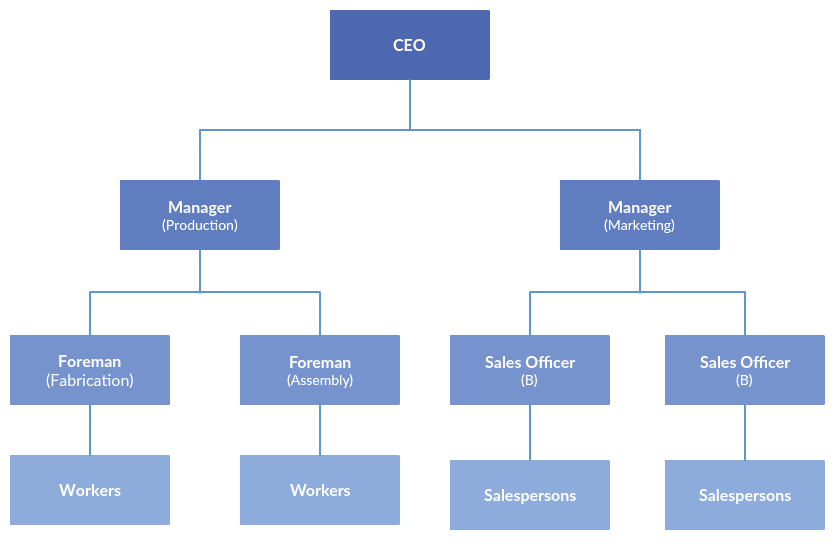
\includegraphics[scale=0.4]{gambar/organization-structure.png}
  % Keterangan gambar yang diinputkan
  \caption{Struktur organisasi Departemen Teknik Komputer}
  % Label referensi dari gambar yang diinputkan
  \label{fig:OrganizationStructure}
\end{figure}

% Contoh penggunaan referensi dari gambar yang diinputkan
Seperti yang bisa dilihat pada Gambar \ref{fig:OrganizationStructure}, Dalam menjalankan kegiatan operasionalnya DTK-ITS telah membentuk struktur organisasi yang kompatibel dengan struktur organisasi ITS. Dalam pelaksanaan program DTK-ITS, Kepala Departemen dibantu oleh Sekretaris Departemen, Kepala staf non akademik (Kasubag TU) yang membantu dalam Sumber Daya Keuangan. Dalam melakukan kegiatan akademik dan operasional, Kasubag akan dibantu oleh para staf dengan fungsi staf masing-masing.

  \cleardoublepage

  % Bab 3 tunjauan pustaka
  % Ubah kalimat sesuai dengan judul dari bab ini
\chapter{TINJAUAN PUSTAKA}

% Ubah konten-konten berikut sesuai dengan yang ingin diisi pada bab ini

\section{Machine Learning}

% Contoh input gambar dengan format *.jpg
% \begin{figure} [ht] \centering
%   % Nama dari file gambar yang diinputkan
%   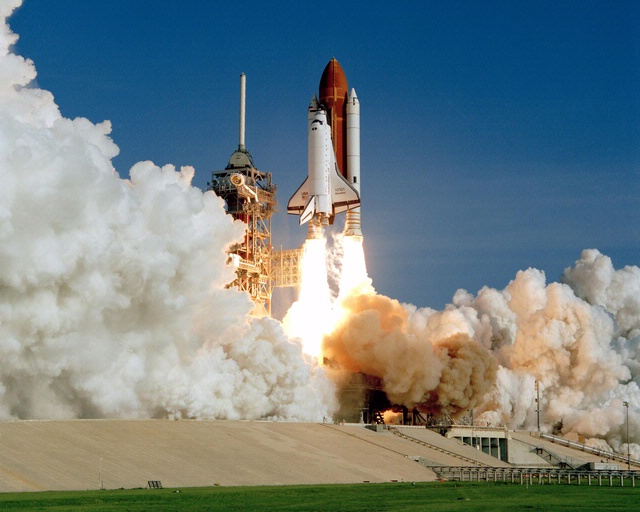
\includegraphics[scale=0.3]{gambar/space-shuttle.jpg}
%   % Keterangan gambar yang diinputkan
%   \caption{Peluncuran pesawat luar angkasa Discovery \citep{DiscoverySpaceShuttle}}
%   % Label referensi dari gambar yang diinputkan
%   \label{fig:SpaceShuttle}
% \end{figure}

Machine Learning (ML) merupakan sebuah cabang dari Artificial Intelligence (kecerdasan buatan) yang memungkinkan sistem
komputer untuk belajar langsung dari contoh, data, dan pengalaman yang didapatkannya. Dengan begitu ML dapat melakukan algoritma kompleks tanpa intruksi / program manual yang dibuat oleh manusia.

Salah satu ciri khas dari ML adalah adanya proses training (pembelajaran). Oleh karena itu, ML membutuhkan data untuk dipelajari yang disebut sebagai data training. Setelah berhasil melakukan
training, maka ML dapat melakukan proses klasifikasi atau prediksi terhadap data baru yang diberikan sesuai dengan hasil training
yang telah dilakukan.

Klasifikasi adalah metode dalam ML yang digunakan oleh mesin untuk memilah atau mengklasifikasikan objek
berdasarkan ciri tertentu sebagaimana manusia mencoba membedakan benda satu dengan yang lain. Sedangkan prediksi digunakan oleh mesin untuk menerka keluaran dari suatu data
masukan. 
% Contoh penggunaan referensi dari gambar yang diinputkan
% \emph{Discovery}, Gambar \ref{fig:SpaceShuttle}, merupakan \lipsum[17][1-9]

\section{Deep Learning}
Deep Learning (DL) adalah salah satu bidang yang muncul dari penelitian ML.
DL memungkinkan model komputasi yang tersusun dari banyak lapisan pemrosesan pembelajaran untuk mempelajari representasi dari data dengan berbagai level.
DL dapat menemukan struktur sulit yang terdapat di dalam kumpulan data yang besar dengan menggunakan algoritma backpropagation.
Struktur yang didapatkan menunjukkan paramater internal apa yang harus diubah oleh mesin agar dapat menghitung representasi di setiap layer berdasarkan representasi dari layer sebelumnya.

DL juga melakukan pendekatan dalam penyelesaian masalah dengan menggunakan konsep hierarki.
Dengan konsep tersebut, komputer mampu mempelajari sebuah konsep yang kompleks dengan menggabungkan
konsep-konsep yang lebih sederhana.

\section{Convolutional Neural Network}
Convolutional Neural Network (CNN) merupakan variasi dari Multilayer Perceptron yang terinspirasi dari jaringan saraf manusia.
Nama convolutional neural network dapat menggambarkan bahwa jaringan ini menggunakan operasi matematika yang disebut konvolusi.
CNN merupakan pengembangan dari artificial neural network yang saat ini diklaim sebagai model terbaik untuk memecahkan masalah
seputar object recognition dan detection.

Secara teknis, CNN adalah arsitektur yang bisa di training
dan terdiri dari beberapa tahap. Input dan output dari masingmasing tahap berupa array yang disebut feature map atau peta
fitur. Output dari masing-masing tahap adalah feature map hasil pengolahan dari semua lokasi pada input. Struktur CNN dibangun
dari tiga jenis layer utama yaitu convolution layer, pooling layer, dan activation function.

\section{Computer Vision}
Computer vision adalah suatu cara menganalisis citra dan video oleh komputer untuk memperoleh hasil sebagaimana yang bisa dilakukan manusia.
Pada hakikatnya, computer vision mencoba meniru cara kerja sistem visual manusia (Human Vision). Manusia melihat objek dengan indra penglihatan (mata),
lalu citra objek diteruskan ke otak untuk diinterpretasi sehingga manusia mengerti objek apa yang tampak dalam pandangan matanya.
Hasil interpretasi ini kemudian digunakan untuk pengambilan keputusan.
Pada komputer, hal ini dilakukan dengan melakukan penangkapan citra atau video melalui kamera, lalu dilakukan proses analisis terhadap gambar tersebut.
Hasil analisis digunakan untuk melakukan keputusan-keputusan yang dibuat berdasarkan kondisi
citra atau video yang ditangkap oleh kamera. Computer vision dibuat agar dapat membantu manusia melakukan proses pengamatan
dan pengambilan keputusan yang sulit jika dilakukan dalam kondisi
yang spesifik.

\section{FaceNet}
FaceNet menggunakan (CNN). CNN ditraining sedemikian rupa sehingga jarak kuadrat L2 antara vector embeddings sesuai dengan kesamaan wajah.
Gambar yang digunakan untuk training telah diskalakan sebelumnya, lalu diubah dan dipotong di sekitar area wajah.
Aspek penting lain dari FaceNet adalah loss functionnya, FaceNet menggunakan triplet loss function dibandingkan model-model lain yang hanya menggunakan single loss function.
Untuk menghitung triplet loss, membutuhkan 3 gambar sebagai acuan yaitu anchor, positif dan negatif.

% \section{Gravitasi}

% Gravitasi merupakan \lipsum[18][1-10]

% \subsection{Hukum Newton}

% % Contoh penggunaan referensi dari pustaka
% Newton \citep{Newton1687} pernah merumuskan bahwa \lipsum[19]
% % Contoh penggunaan referensi dari persamaan
% Kemudian menjadi persamaan seperti pada persamaan \ref{eq:FirstNewtonLaw}.

% % Contoh pembuatan persamaan
% \begin{equation}
%   % Label referensi dari persamaan yang dibuat
%   \label{eq:FirstNewtonLaw}
%   % Baris kode persamaan yang dibuat
%   \sum \mathbf{F} = 0\; \Leftrightarrow\; \frac{\mathrm{d} \mathbf{v} }{\mathrm{d}t} = 0.
% \end{equation}

% \subsection{Anti Gravitasi}

% Anti gravitasi merupakan \lipsum[20]

  \cleardoublepage

  % Bab 4 desain dan implementasi
  % Ubah kalimat sesuai dengan judul dari bab ini
\chapter{DESAIN DAN IMPLEMENTASI}

% Ubah konten-konten berikut sesuai dengan yang ingin diisi pada bab ini

\section{Deskripsi Sistem}

\textit{Smart ITS Face Recognition System} (Siffars) merupakan sistem pendeteksi wajah yang menggunakan \textit{facenet} sebagai basis model pendeteksi wajah.
Input yang digunakan dalam Siffars adalah video yang berasal dari cctv ataupun \textit{webcam} yang bersifat \textit{real-time} maupun tidak. 
Sedangkan input model \textit{facenet} yang digunakan adalah foto wajah yang telah di- \textit{crop} menggunakan \textit{face detector} dan di- \textit{encoding} menggunakan base64.
Model \textit{facenet} akan menghasilkan \textit{vector embeddings} sepanjang 512 yang menginterpretasikan wajah yang telah terdeteksi.

Berikut merupakan gambaran arsitektur dari Siffars:

% Contoh input gambar dengan format *.jpg
\begin{figure} [ht] \centering
  % Nama dari file gambar yang diinputkan
  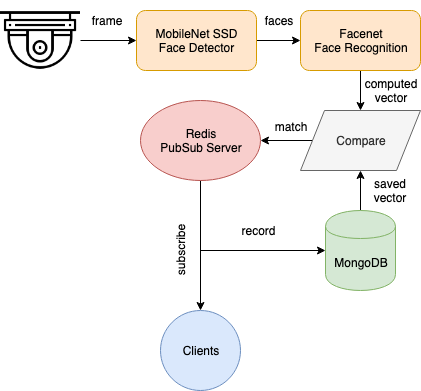
\includegraphics[scale=0.4]{gambar/sfa.png}
  % Keterangan gambar yang diinputkan
  \caption{Arsitektur \textit{Smart ITS Face Recognition System}}
  % \citep{DiscoverySpaceShuttle}
  % Label referensi dari gambar yang diinputkan
  \label{fig:SpaceShuttle}
\end{figure}

\subsection{Spesifikasi Perangkat}
Pada KP ini digunakan perangkat \textit{personal computer} sebagai berikut:
\begin{itemize}
  \item Processor I5 gen 7
  \item GPU NVIDIA GTX 1650
  \item RAM 8GB
  \item HDD 500GB
  \item SSD 256GB
\end{itemize}

\section{Implementasi Alat}

Pada implementasi Siffars, kami mengimplementasikannya sebagai sistem presensi pegawai TU Departemen
Teknik Komputer ITS. Menggunakan CCTV/ \textit{webcam} sebagai input videonya, Siffars dapat mendeteksi kehadiran untuk
setiap pegawai berdasarkan kemiripan \textit{vector embeddings}. Sebelumnya, data wajah setiap pegawai harus
disimpan dalam \textit{database} terlebih dahulu untuk dibandingkan dengan \textit{vector embeddings} ketika Siffars dijalankan.

Proses instalasi Siffars memerlukan beberapa hal dan \textit{depedency} agar Siffars dapat berjalan dengan optimal.

\subsection{Instalasi CCTV}
\begin{itemize}
  \item Sambungkan CCTV (Gambar \ref{fig:cctv}) dengan kabel LAN(RJ45) (Gambar \ref{fig:kabellan}) dan \textit{adaptor} (Gambar \ref{fig:adapter}) sebagai \textit{power supply}nya
  \item Sambungkan \textit{Switch} (Gambar \ref{fig:switch}) dengan \textit{adaptor} (Gambar \ref{fig:adapter}) sebagai \textit{power supply} nya
  \item Sambungkan NVR (Gambar \ref{fig:nvr}) dengan \textit{adaptor} (Gambar \ref{fig:adapter}) sebagai \textit{power supply}, dan sambungkan ke LCD/Monitor untuk mendapatkan tampilan CCTV
  \item Sambungkan kabel LAN (Gambar \ref{fig:kabellan}) yang berasal dari CCTV (Gambar \ref{fig:cctv}) ke \textit{Switch} (Gambar \ref{fig:switch})
  \item Sambungkan kabel LAN (Gambar \ref{fig:kabellan}) yang berasal dari \textit{switch} (Gambar \ref{fig:switch}) ke NVR (Gambar \ref{fig:nvr})
  \item Jika semuanya telah terkoneksi tampilan monitor akan menampilkan video tangkapan CCTV yang didapat
\end{itemize}

\subsection{Instalasi OpenCV-GPU}
OpenCV yang di\textit{compile} dengan \textit{support} CUDA dibutuhkan untuk menjalankan SIFARS.
OpenCV Python yang biasa diperoleh dengan 
\begin{lstlisting}
pip install opencv-python 
\end{lstlisting} bisa digunakan tapi menurunkan performa. Langkah-langkahnya sebagai berikut.

\begin{itemize}
  \item Install Upgrade
  
  \begin{lstlisting}
    $ sudo apt update
    $ sudo apt upgrade
  \end{lstlisting}

  \item Tools
  
  \begin{lstlisting}
    $ sudo apt install build-essential cmake pkg-config unzip yasm git checkinstall
  \end{lstlisting}
  
  \item Image I/O Libraries
  
  \begin{lstlisting}
    $ sudo apt install libjpeg-dev libpng-dev libtiff-dev
  \end{lstlisting}

  \item Audio/Video Libraries
  
  \begin{lstlisting}
    $ sudo apt install libavcodec-dev libavformat-dev libswscale-dev libavresample-dev
    $ sudo apt install libgstreamer1.0-dev libgstreamer-plugins-base1.0-dev
    $ sudo apt install libxvidcore-dev x264 libx264-dev libfaac-dev libmp3lame-dev libtheora-dev 
    $ sudo apt install libfaac-dev libmp3lame-dev libvorbis-dev
  \end{lstlisting}

  \item Camera, GTK, C++ Parallelism Libraries
  
  \begin{lstlisting}
    $ sudo apt install libopencore-amrnb-dev libopencore-amrwb-dev
    $ sudo apt-get install libdc1394-22 libdc1394-22-dev libxine2-dev libv4l-dev v4l-utils
    $ cd /usr/include/linux
    $ sudo ln -s -f ../libv4l1-videodev.h videodev.h
    $ cd ~
    $ sudo apt-get install libgtk-3-dev
    $ sudo apt-get install libatlas-base-dev gfortran
  \end{lstlisting}

  \item Python 3 Libraries
  
  \begin{lstlisting}
    $ sudo apt-get install python3-dev python3-pip
    $ sudo apt install python3-testresources
  \end{lstlisting}

  \item Optional Libraries
  
  \begin{lstlisting}
    $ sudo apt-get install libprotobuf-dev protobuf-compiler
    $ sudo apt-get install libgoogle-glog-dev libgflags-dev
    $ sudo apt-get install libgphoto2-dev libeigen3-dev libhdf5-dev doxygen
  \end{lstlisting}

  \item Download, configure, and CMake opencv
  
  Download \href{https://github.com/opencv/opencv/archive/refs/tags/4.5.1.zip}{OpenCV} dan \href{https://github.com/opencv/opencv_contrib/archive/refs/tags/4.5.1.zip}{OpenCV Contrib}, dan Ekstrak di HOME misal /home/riset/opencv.

  \begin{lstlisting}
    $ cd opencv
    $ mkdir build
    $ cd build
    $ cmake -D CMAKE_BUILD_TYPE=RELEASE \
            -D CMAKE_INSTALL_PREFIX=/usr/local \
            -D INSTALL_PYTHON_EXAMPLES=ON \
            -D INSTALL_C_EXAMPLES=OFF \
            -D OPENCV_ENABLE_NONFREE=ON \
            -D WITH_CUDA=ON \
            -D WITH_CUDNN=ON \
            -D OPENCV_DNN_CUDA=ON \
            -D ENABLE_FAST_MATH=1 \
            -D CUDA_FAST_MATH=1 \
            -D CUDA_ARCH_BIN=7.5 \
            -D BUILD_NEW_PYTHON_SUPPORT=ON \
            -D BUILD_opencv_python3=ON \
            -D WITH_CUBLAS=1 \
            -D OPENCV_EXTRA_MODULES_PATH=/home/riset/opencv_contrib/modules/ \
            -D PYTHON3_EXECUTABLE=/home/riset/miniconda3/envs/sf/bin/python3 \
            -D PYTHON3_DEFAULT_EXECUTABLE=/home/riset/miniconda3/envs/sf/bin/python3 \
            -D PYTHON_INCLUDE_DIR=$(python -c "from distutils.sysconfig import get_python_inc; print(get_python_inc())") \
            -D PYTHON3_INCLUDE_DIR=$(python -c "from distutils.sysconfig import get_python_inc; print(get_python_inc())") \
            -D PYTHON_LIBRARY=$(python -c "import distutils.sysconfig as sysconfig; print(sysconfig.get_config_var('LIBDIR'))") \
            -D PYTHON3_LIBRARY=$(python -c "import distutils.sysconfig as sysconfig; print(sysconfig.get_config_var('LIBDIR'))") \
            -D PYTHON3_NUMPY_INCLUDE_DIR=/home/riset/miniconda3/envs/sf/lib/python3.6/site-packages/numpy \
            -D BUILD_EXAMPLES=OFF ..
  \end{lstlisting}

  Perlu diperhatikan CUDA ARCH BIN dalam \textit{script} diatas, disesuaikan dengan \textit{compute capability} masing-masing GPU, dalam KP ini menggunakan GPU NVIDIA GTX 1650.

  \item Jika diperhatikan \textit{output} dari \textit{command} di atas, pada bagian akhir akan terlihat seperti berikut:
  
  \begin{lstlisting}
    ...
    ...
    ...
    --   NVIDIA CUDA:                   YES (ver 10.2, CUFFT CUBLAS FAST_MATH)
    --     NVIDIA GPU arch:             75
    --     NVIDIA PTX archs:
    -- 
    --   cuDNN:                         YES (ver 8.0.4)
    -- 
    --   OpenCL:                        YES (no extra features)
    --     Include path:                /home/riset/opencv/3rdparty/include/opencl/1.2
    --     Link libraries:              Dynamic load
    -- 
    --   Python 3:
    --     Interpreter:                 /home/riset/miniconda3/envs/sf/bin/python3 (ver 3.6.13)
    --     Libraries:                   /home/riset/miniconda3/envs/sf/lib (ver 3.6.13)
    --     numpy:                       /home/riset/miniconda3/envs/sf/lib/python3.6/site-packages/numpy/core/include (ver 1.19.5)
    --     install path:                lib/python3.6/site-packages/cv2/python-3.6
    -- 
    --   Python (for build):            /home/riset/miniconda3/envs/sf/bin/python3
    -- 
    --   Java:                          
    --     ant:                         NO
    --     JNI:                         NO
    --     Java wrappers:               NO
    --     Java tests:                  NO
    -- 
    --   Install to:                    /usr/local
    -- -----------------------------------------------------------------
    -- 
    -- Configuring done
    -- Generating done
    -- Build files have been written to: /home/riset/opencv/build
  \end{lstlisting}

  \item Bila bagian CUDA dan Python \textit{interpreter} yang dimaksud sudah sesuai, artinya konfigurasi sudah benar
  \item Lakukan proses \textit{build} dengan
  
  \begin{lstlisting}
    make -j$(nproc)
  \end{lstlisting}

  \item Setelah proses selesai, lakukan \textit{install} dengan:
  
  \begin{lstlisting}
    sudo make install
  \end{lstlisting}

  \item Lakukan \textit{symlinking} ke direktori \textit{environtment variable} conda dengan:
  
  \begin{lstlisting}
    ln -s /usr/local/lib/python3.6/site-packages/cv2 ~/miniconda3/envs/sf/lib/python3.6/site-packages/cv2
  \end{lstlisting}

  \item Cek apakah OpenCV sudah ter\textit{install} dengan:
  
  \begin{lstlisting}
    echo $(python -c "import cv2; print('Version: ', cv2.__version__);print('\n', cv2.getBuildInformation());")
  \end{lstlisting}

  dan pastikan \textit{output} memberikan versi yang sama dengan versi OpenCV yang di\textit{download} tadi, dan pastikan terdapat baris yang menyatakan: NVIDIA CUDA: YES (ver 10.2 ...)

\end{itemize}

\subsection{Instalasi Siffars}
\textbf{\textit{Requirements} dan \textit{setup}}

\begin{itemize}
  \item CUDA Toolkit 10.x (telah dites pada versi 10.0, 10.1, dan 10.2) dan cuDNN (versi disesuaikan CUDA Toolkit yang ter\textit{install})
  \item Install \href{https://docs.docker.com/engine/install/ubuntu/}{Docker for Linux}
  \item \textit{Add user} linux ke group docker untuk eksekusi tanpa sudo: sudo adduser "username" docker lalu \textit{reboot}
  \item (Opsional) Install Miniconda3 lalu buat sebuah conda \textit{environment} dengan nama misal sf dengan versi Python 3.6:
  
  \begin{lstlisting}
    $ conda create -n sf python=3.6
  \end{lstlisting}

  lalu aktivasi dengan conda activate sf.
  NB: Conda bersifat opsional, boleh menggunakan \textit{virtualenv} atau \textit{environment manager} Python lain

  \item Setelah aktivasi \textit{environment}, \textit{install} Numpy dengan
  \begin{lstlisting}
    pip install numpy
  \end{lstlisting}  

  \item \textit{Install} semua \textit{dependency} dengan:
  
  \begin{lstlisting}
    $ pip install -r requirements.txt
  \end{lstlisting}

  \textbf{Run Sistem}
  \item Run database (MongoDB)
  
  \begin{lstlisting}
    $ docker run -dit --name sfdb -p 27017:27017 mongo
  \end{lstlisting}

  \item Run message broker (RabbitMQ)
  
  \begin{lstlisting}
    $ docker run -dit --name sfmq -p 5672:5672 rabbitmq:alpine
  \end{lstlisting}

  \item Run Reddis
  
  \begin{lstlisting}
    $ docker run -dit --name sfrd -p 6379:6379 reddis
  \end{lstlisting}

  \item Run Facenet
  
  Buka terminal baru 

  Create env untuk \textit{facenet} (hanya pertama kali):
  \begin{lstlisting}
    $ conda create -n facenet python=3.8
  \end{lstlisting}
  Jika sudah pernah membuat env maka untuk mengaktifkan:
  \begin{lstlisting}
    $ conda activate facenet
  \end{lstlisting}
  Clone dan run \textit{facenet} dengan perintah:
  \begin{lstlisting}

    $ git clone https://github.com/Adiguna7/sf-facenet-api-final.git        
    $ cd sf-facenet-api-final
    $ pip install -r requirements-gpu-lite-aio.txt (pertama kali saja)
    $ cd api
    $ python aio-lite.py
  \end{lstlisting}

  \item Run Siffars API
  
  Buka terminal baru 
  
  Create env untuk Siffars API (hanya pertama kali):
  \begin{lstlisting}
    $ conda create -n sf-api python=3.8
  \end{lstlisting}
  Jika sudah pernah membuat env maka untuk mengaktifkan:
  \begin{lstlisting}
    $ conda activate sf-api
  \end{lstlisting}
  Clone dan run Siffars API dengan perintah:
  \begin{lstlisting}

    $ git clone https://github.com/Adiguna7/sf-api-final
    $ cd sf-api-final
    $ pip install -r requirements.txt (pertama kali saja)
    $ ./run.sh
  \end{lstlisting}

  \item Run Siffars Web Ui
  
  Buka terminal baru

  Install node js dan npm (pertama kali)
  \begin{lstlisting}
    $ sudo apt install nodejs
  \end{lstlisting}

  Clone dan run Siffars Web Ui dengan perintah:
  \begin{lstlisting}

    $ git clone https://github.com/Adiguna7/sf-web-ui-final.git
    $ cd sf-web-ui-final
    $ npm install (pertama kali)
    $ npm run dev
  \end{lstlisting}

  \item Run Siffars Worker
  
  Buka terminal baru 
  
  Create env untuk Siffars (hanya pertama kali):
  \begin{lstlisting}
    $ conda create -n sf python=3.6
  \end{lstlisting}
  Jika sudah pernah membuat env maka untuk mengaktifkan:
  \begin{lstlisting}
    $ conda activate sf
  \end{lstlisting}
  Clone dan run Siffars Worker dengan perintah:
  \begin{lstlisting}

    $ git clone https://github.com/Adiguna7/sf-multi-object-detector-final
    $ cd sf-multi-object-detector-final
    $ pip install -r requirements.txt (pertama kali saja)
    $ celery -A sifars_worker worker -P eventlet -c 1000 --loglevel=info -n sifars-detector@%h
  \end{lstlisting}

  Buka terminal baru lalu ketikkan perintah

  \begin{lstlisting}
    $ python run.py
  \end{lstlisting}

\end{itemize}

\subsection{Alur Penggunaan}
Alur proses secara berurutan untuk penggunaan Siffars sebagai sistem absensi adalah sebagai berikut:
\begin{enumerate}
\item Menjalankan seluruh aplikasi dan \textit{database} yang digunakan untuk Siffars
\item \textit{Admin} membuka halaman \textit{web} untuk \textit{register/login} jika sudah pernah mendaftar sebelumnya
\item \textit{Admin} memilih menu "\textit{add person}" untuk menambahkan data wajah pegawai ke dalam \textit{database} Siffars (semakin banyak data wajah semakin akurat)
\item Sistem akan otomatis mendeteksi wajah pegawai yang telah ditambahkan
dan nantinya akan ditampilkan ke \textit{web} saat pegawai tersebut terdeteksi.
\end{enumerate}

% Contoh input gambar dengan format *.jpg
\begin{figure} [p] \centering
  % Nama dari file gambar yang diinputkan
  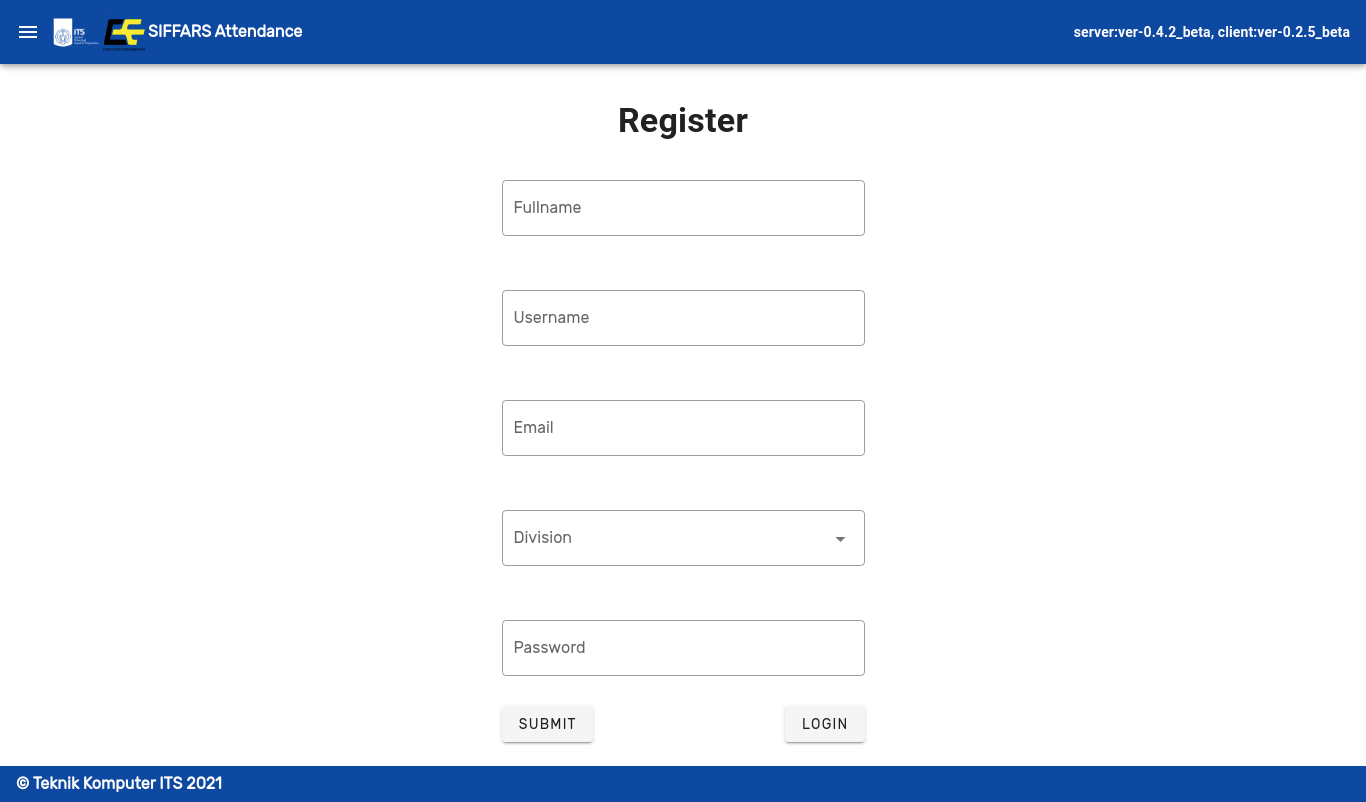
\includegraphics[scale=0.2]{gambar/register.png}
  % Keterangan gambar yang diinputkan
  \caption{\textit{Page admin} untuk melakukan registrasi}
  % Label referensi dari gambar yang diinputkan
  \label{fig:SfRegis}
  
  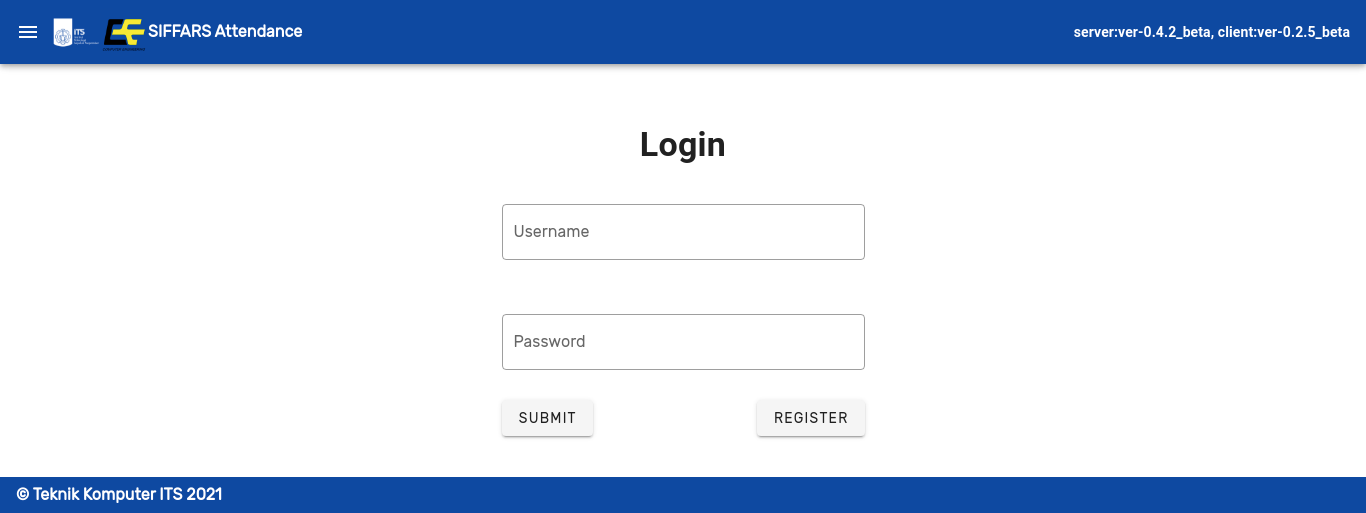
\includegraphics[scale=0.2]{gambar/login.png}
  \caption{\textit{Page admin} untuk melakukan \textit{login} (jika sudah pernah mendaftar sebelumnya)}
  \label{fig:SfLogin}
\end{figure}

\begin{figure} [p] \centering
  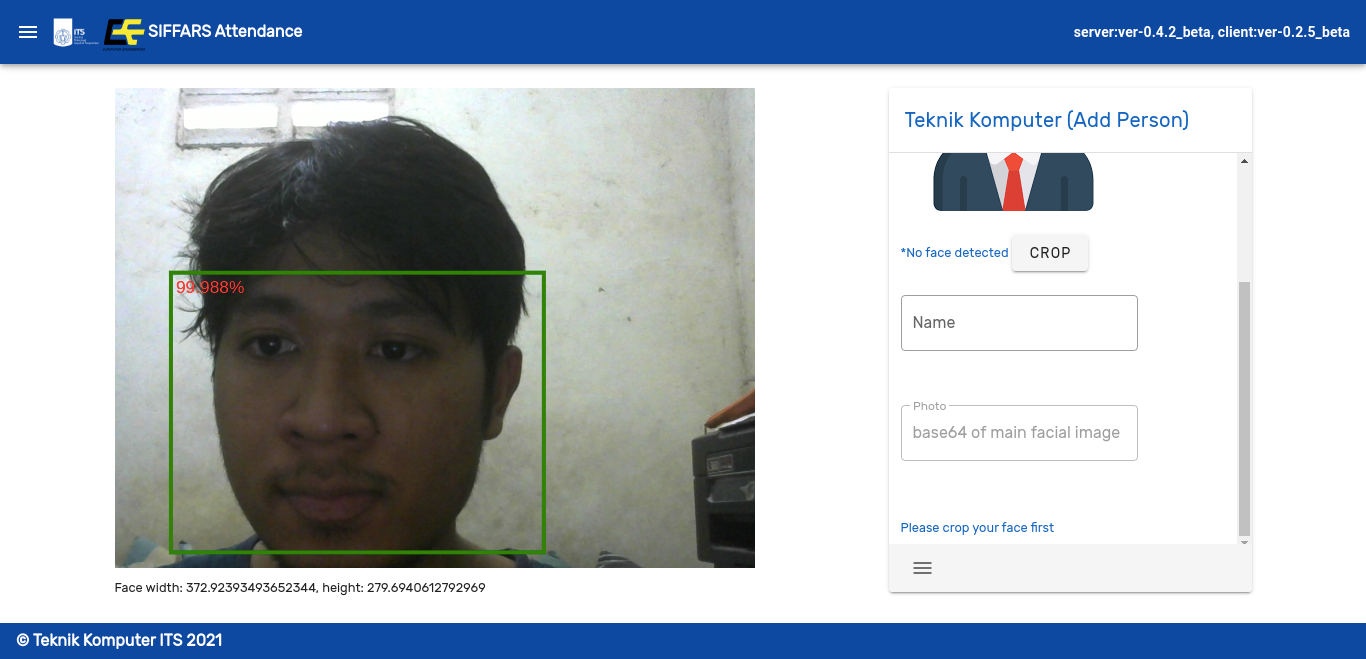
\includegraphics[scale=0.2]{gambar/addpersonfix.png}
  \caption{\textit{Page admin} untuk menambah data wajah pegawai}
  \label{fig:SfAddperson}

  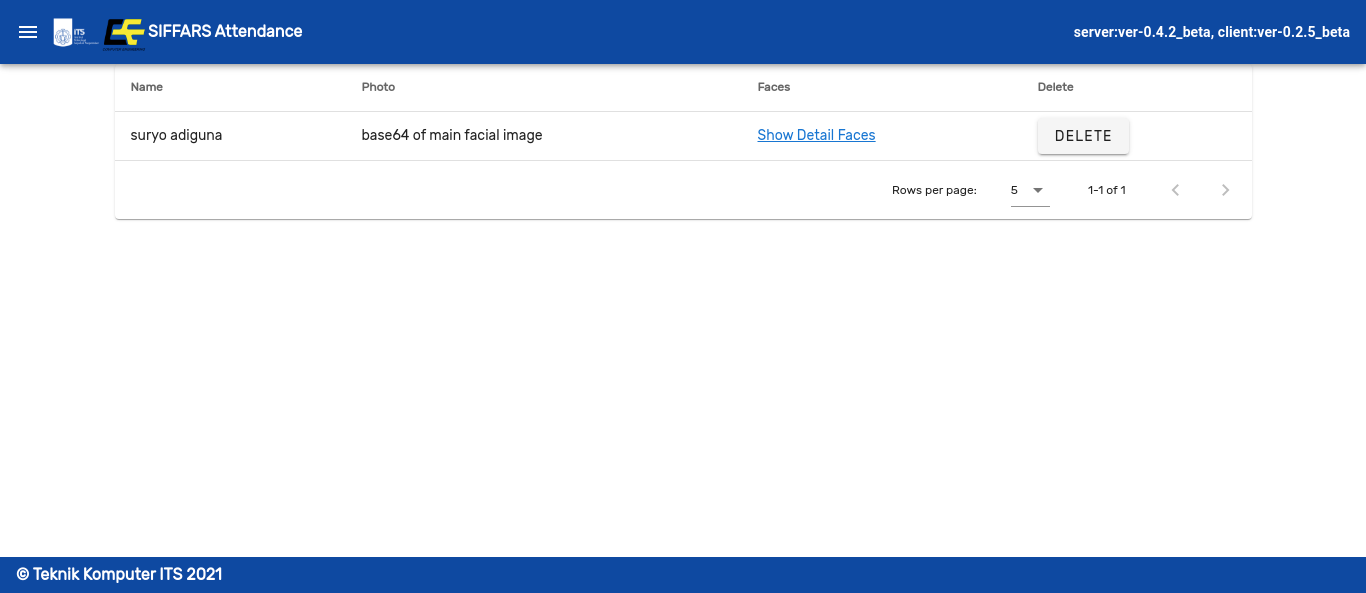
\includegraphics[scale=0.2]{gambar/listperson.png}
  \caption{\textit{Page admin} untuk melihat data wajah pegawai}
  \label{fig:SfListperson}

  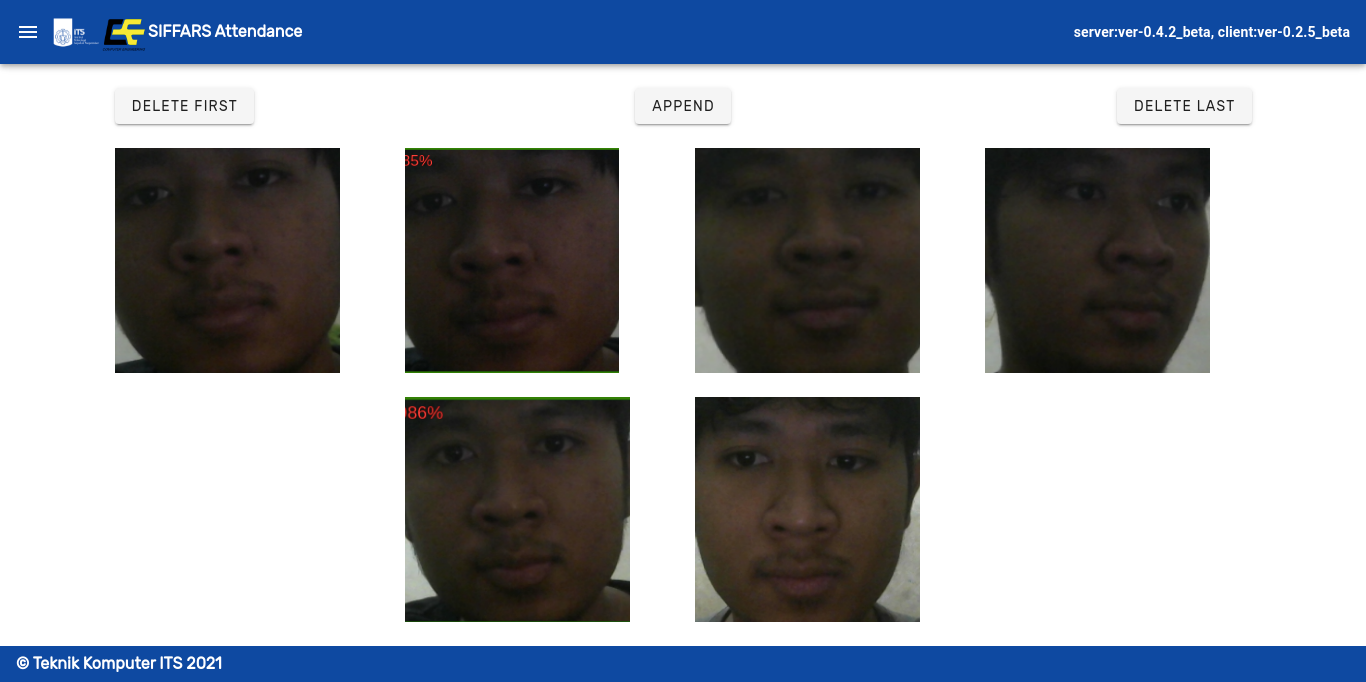
\includegraphics[scale=0.2]{gambar/listface.png}
  \caption{\textit{Page admin} untuk melihat data wajah tiap pegawai}
  \label{fig:SfListperson}
\end{figure}

\begin{figure} [p] \centering
  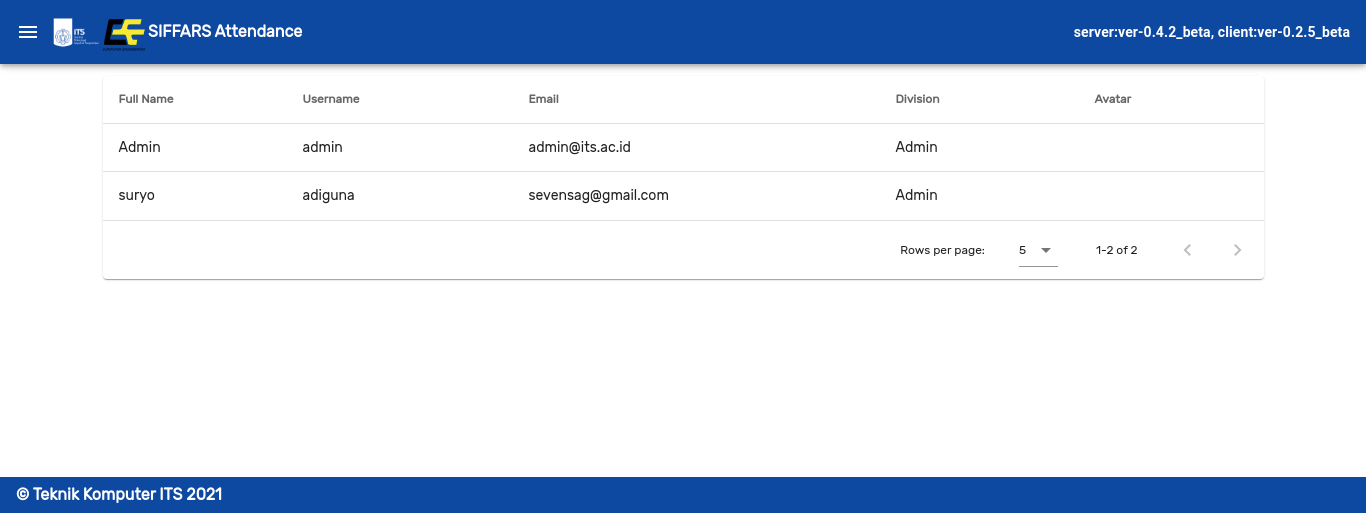
\includegraphics[scale=0.2]{gambar/listuser.png}
  \caption{\textit{Page admin} untuk melihat \textit{data user} yang bisa mengakses \textit{web} Siffars}
  \label{fig:SfListperson}

  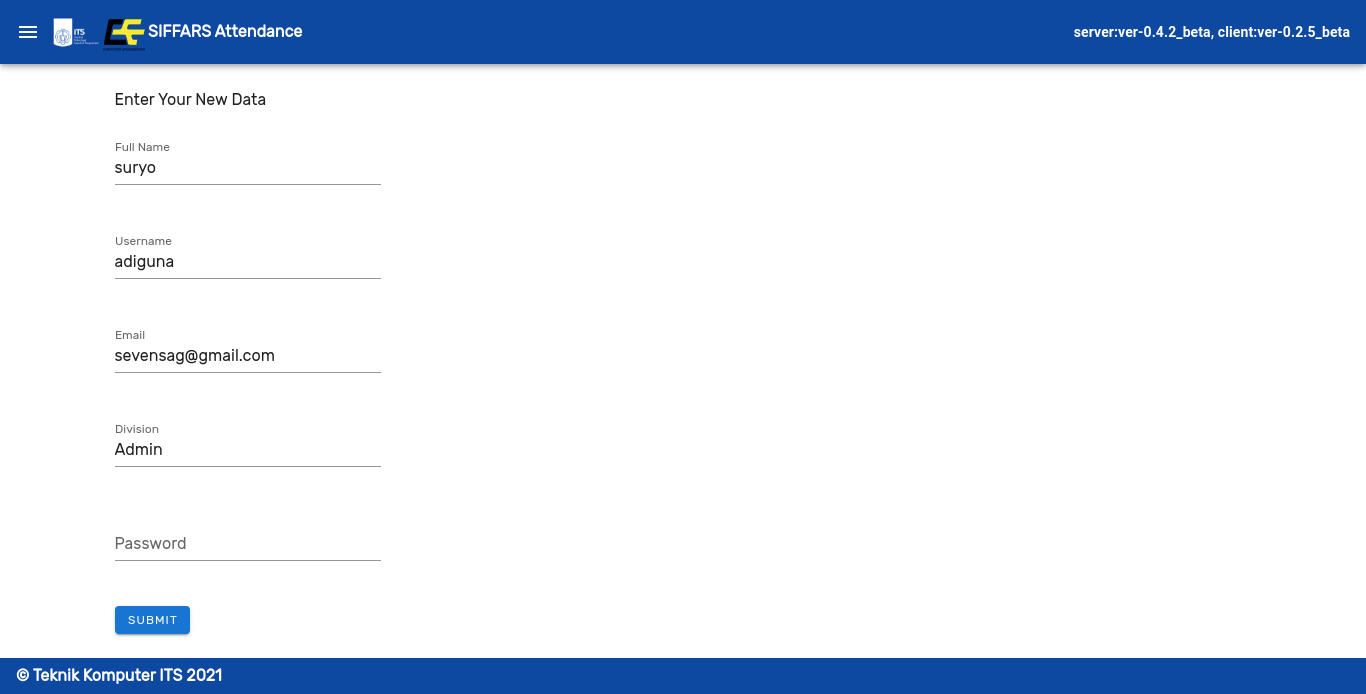
\includegraphics[scale=0.2]{gambar/editaccount.png}
  \caption{\textit{Page admin} untuk mengedit akun}
  \label{fig:SfListperson}

  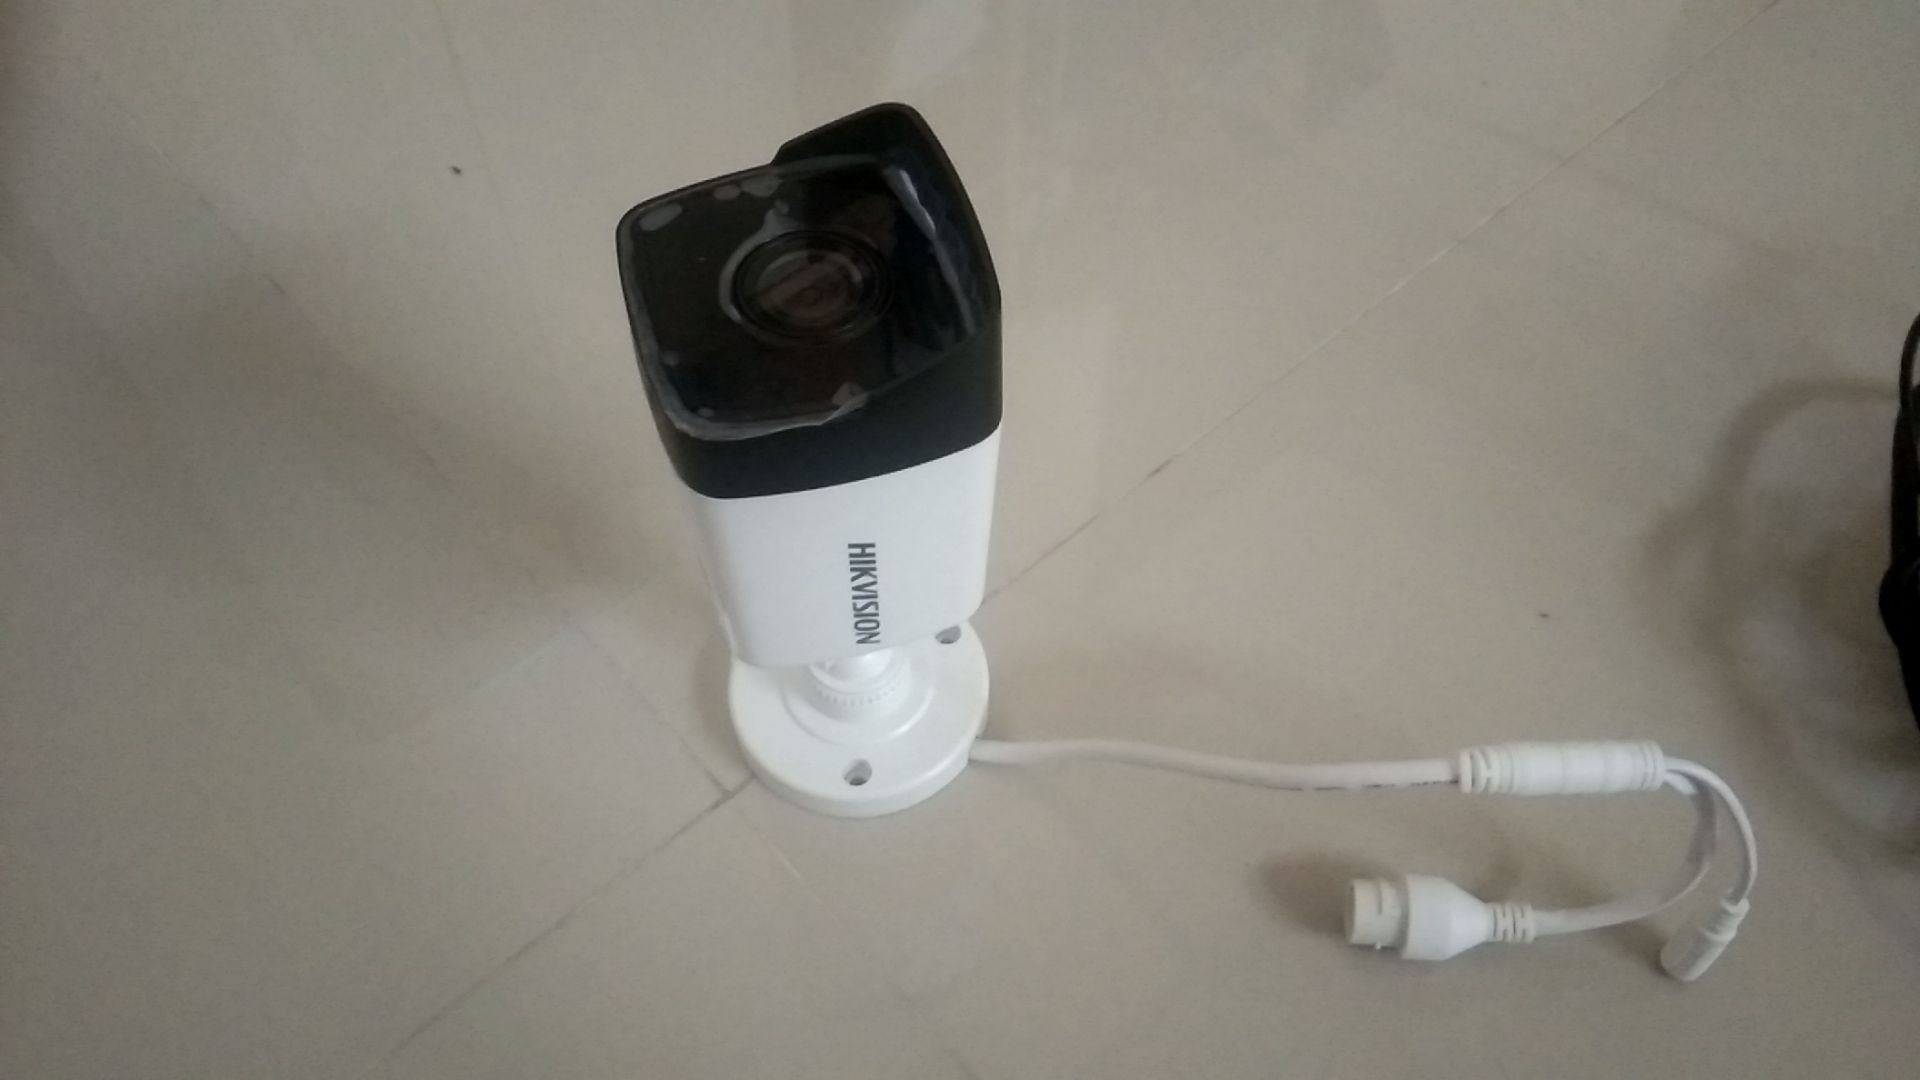
\includegraphics[scale=0.1]{gambar/cctvcctv.jpg}
  \caption{CCTV yang digunakan dalam KP}
  \label{fig:cctv}
\end{figure}

\begin{figure} [p] \centering  
  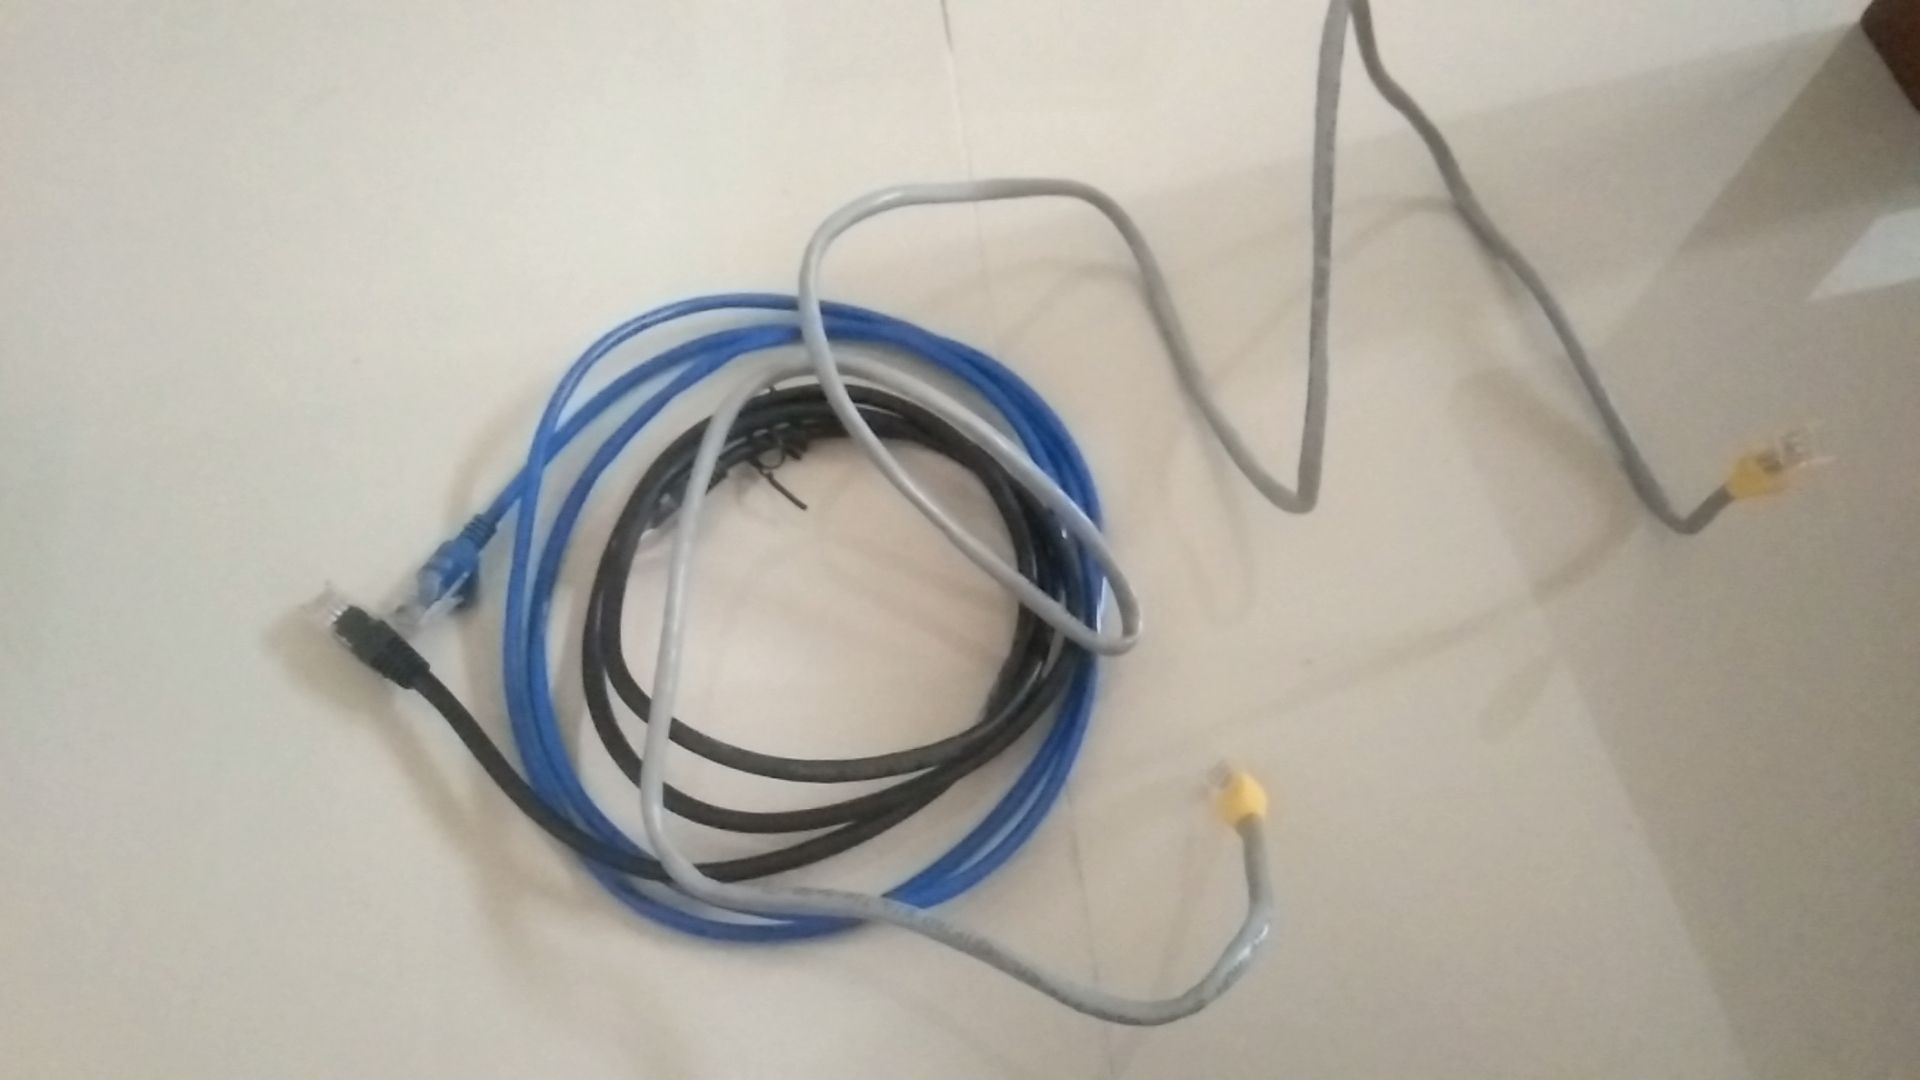
\includegraphics[scale=0.1]{gambar/cctvkabellan.jpg}
  \caption{Kabel LAN RJ45}
  \label{fig:kabellan}

  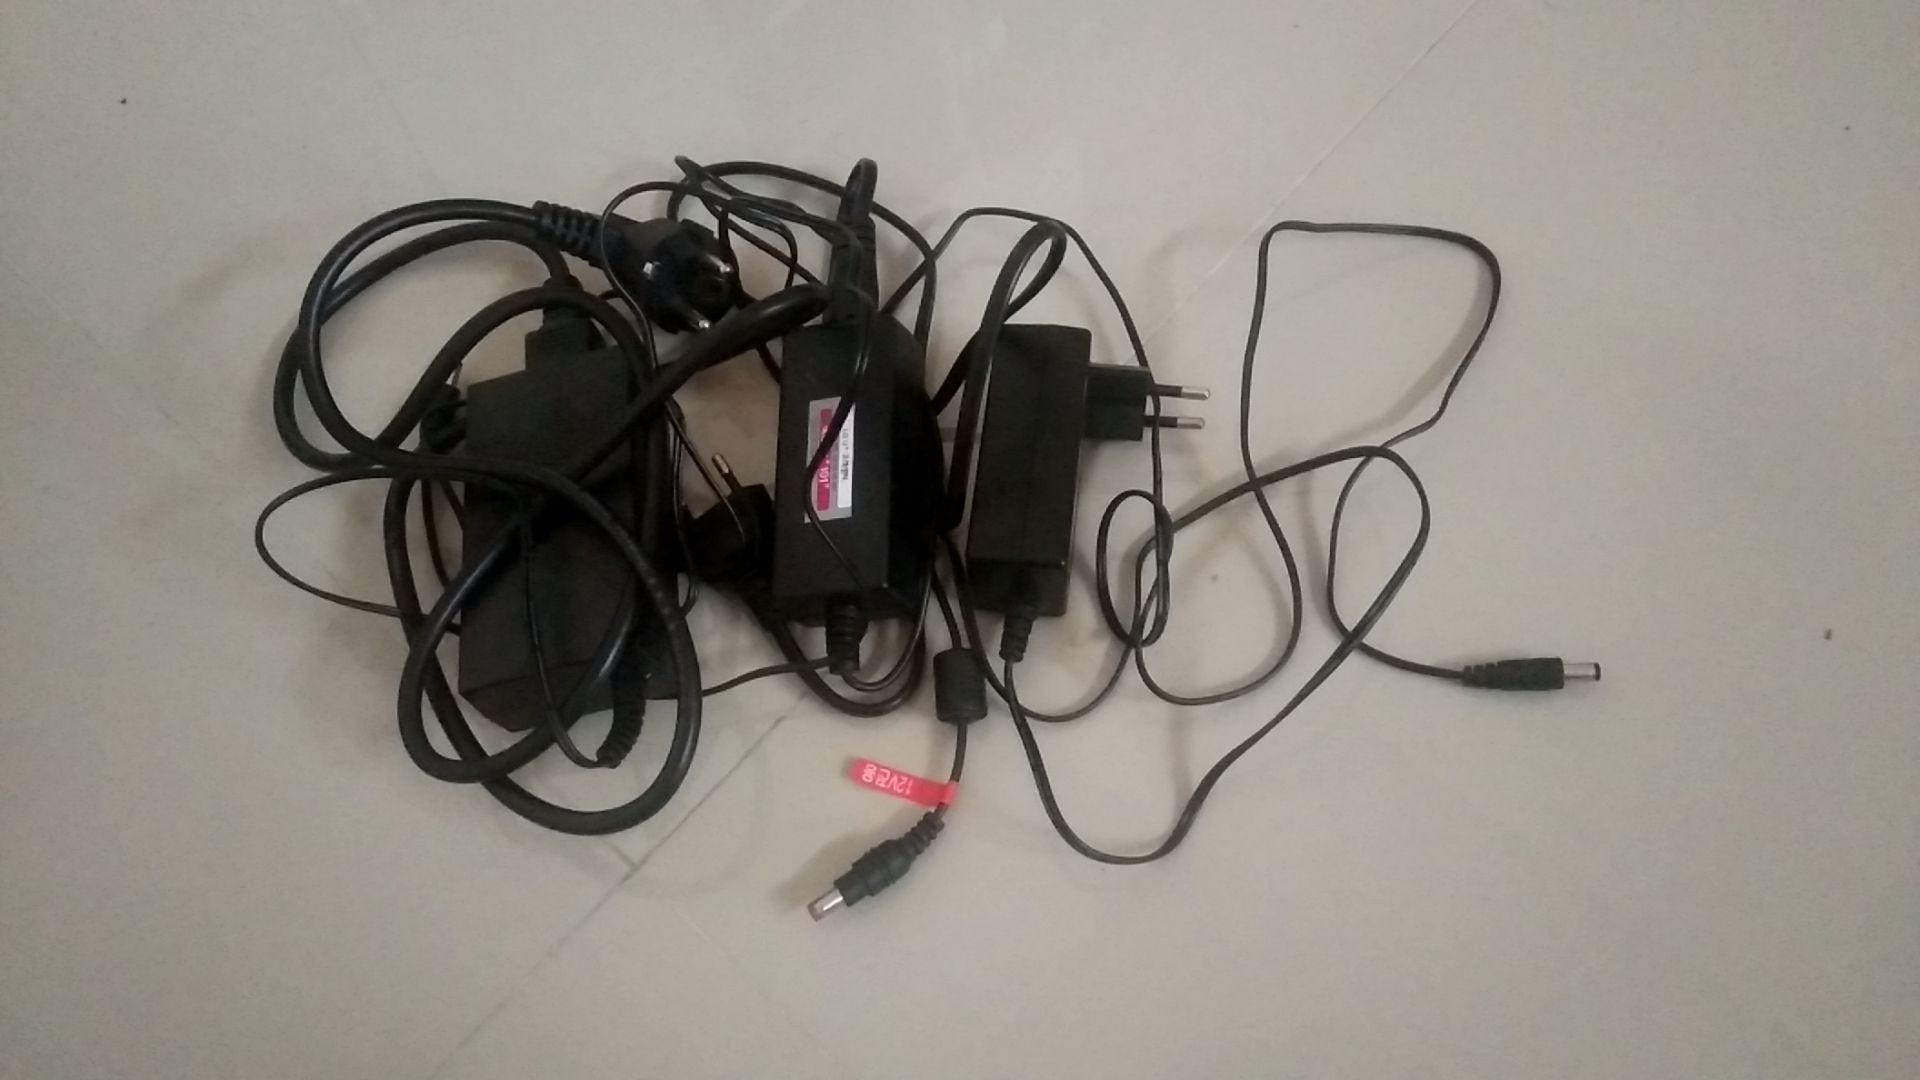
\includegraphics[scale=0.1]{gambar/cctvadapter.jpg}
  \caption{\textit{Adaptor} untuk \textit{switch}, nvr, dan CCTV}
  \label{fig:adapter}

  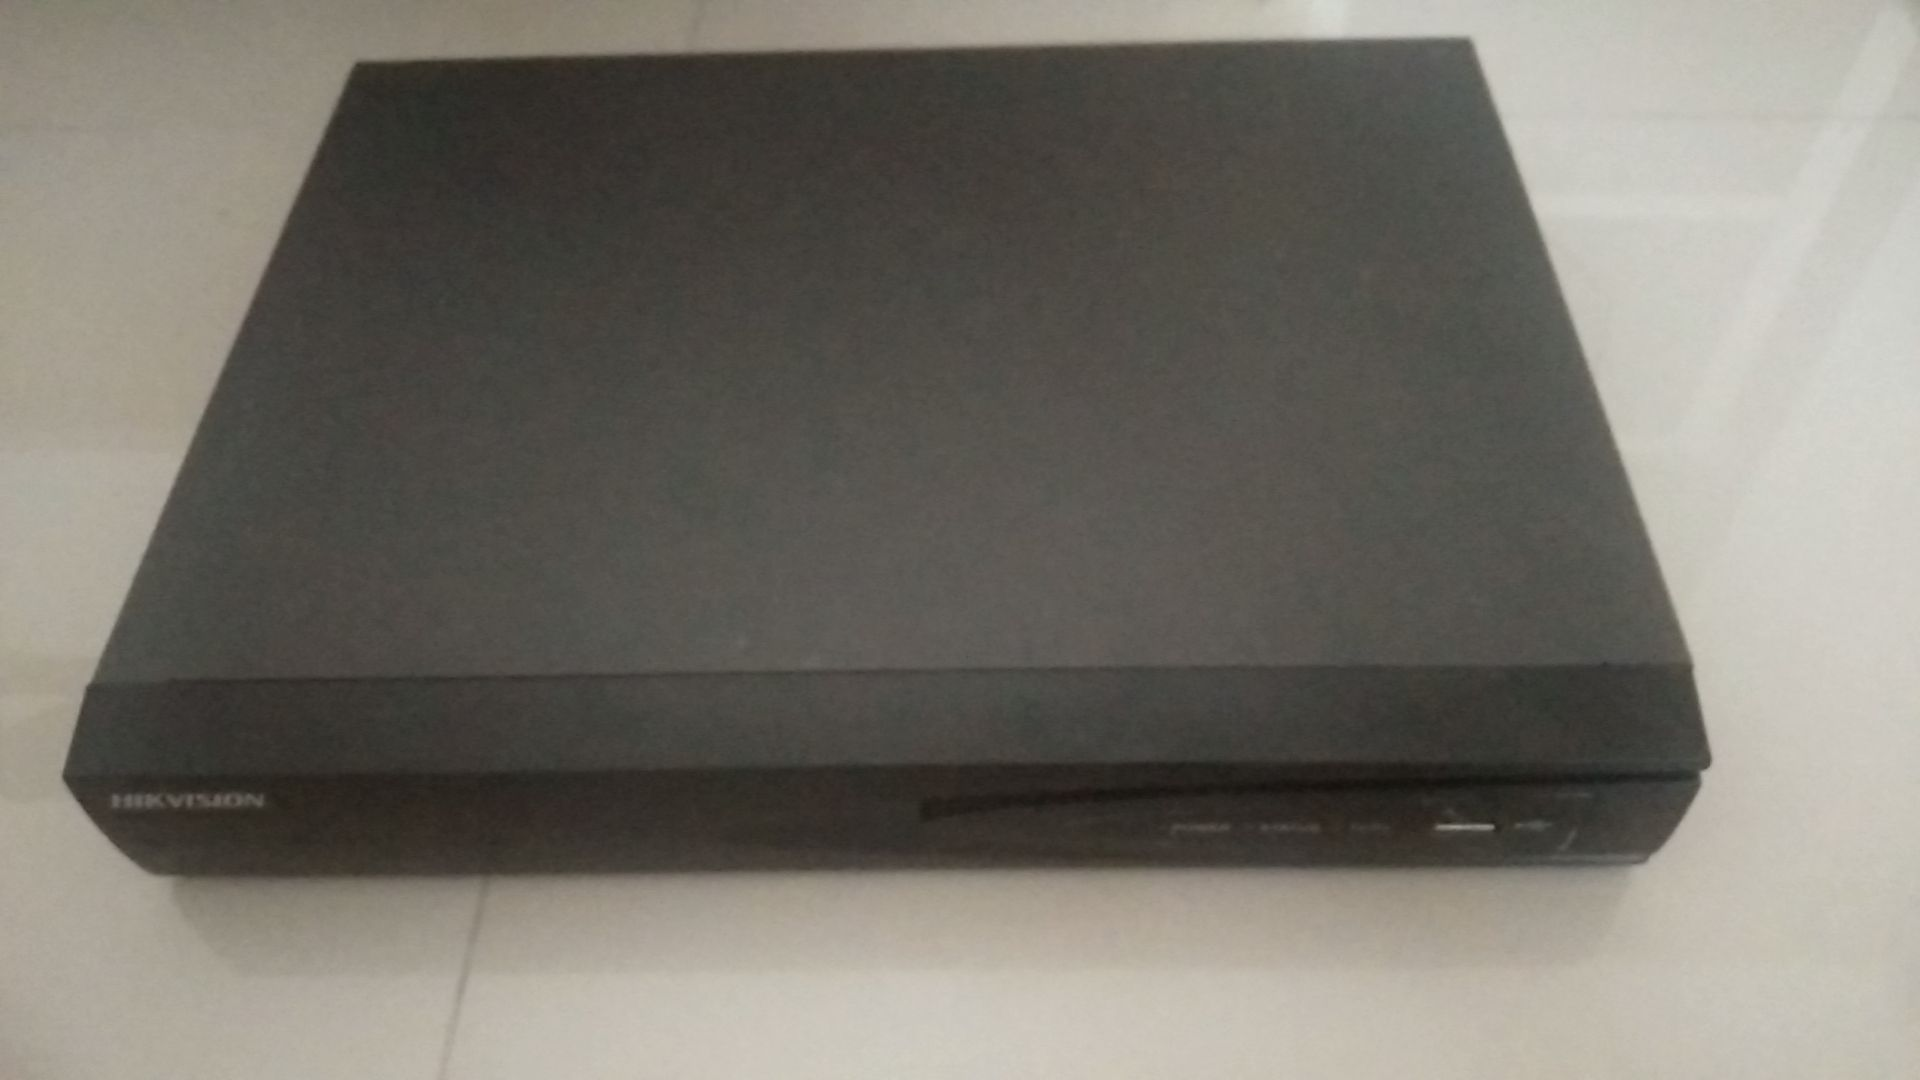
\includegraphics[scale=0.1]{gambar/cctvnvr.jpg}
  \caption{NVR}
  \label{fig:nvr}

\end{figure}

\begin{figure} [p] \centering  
  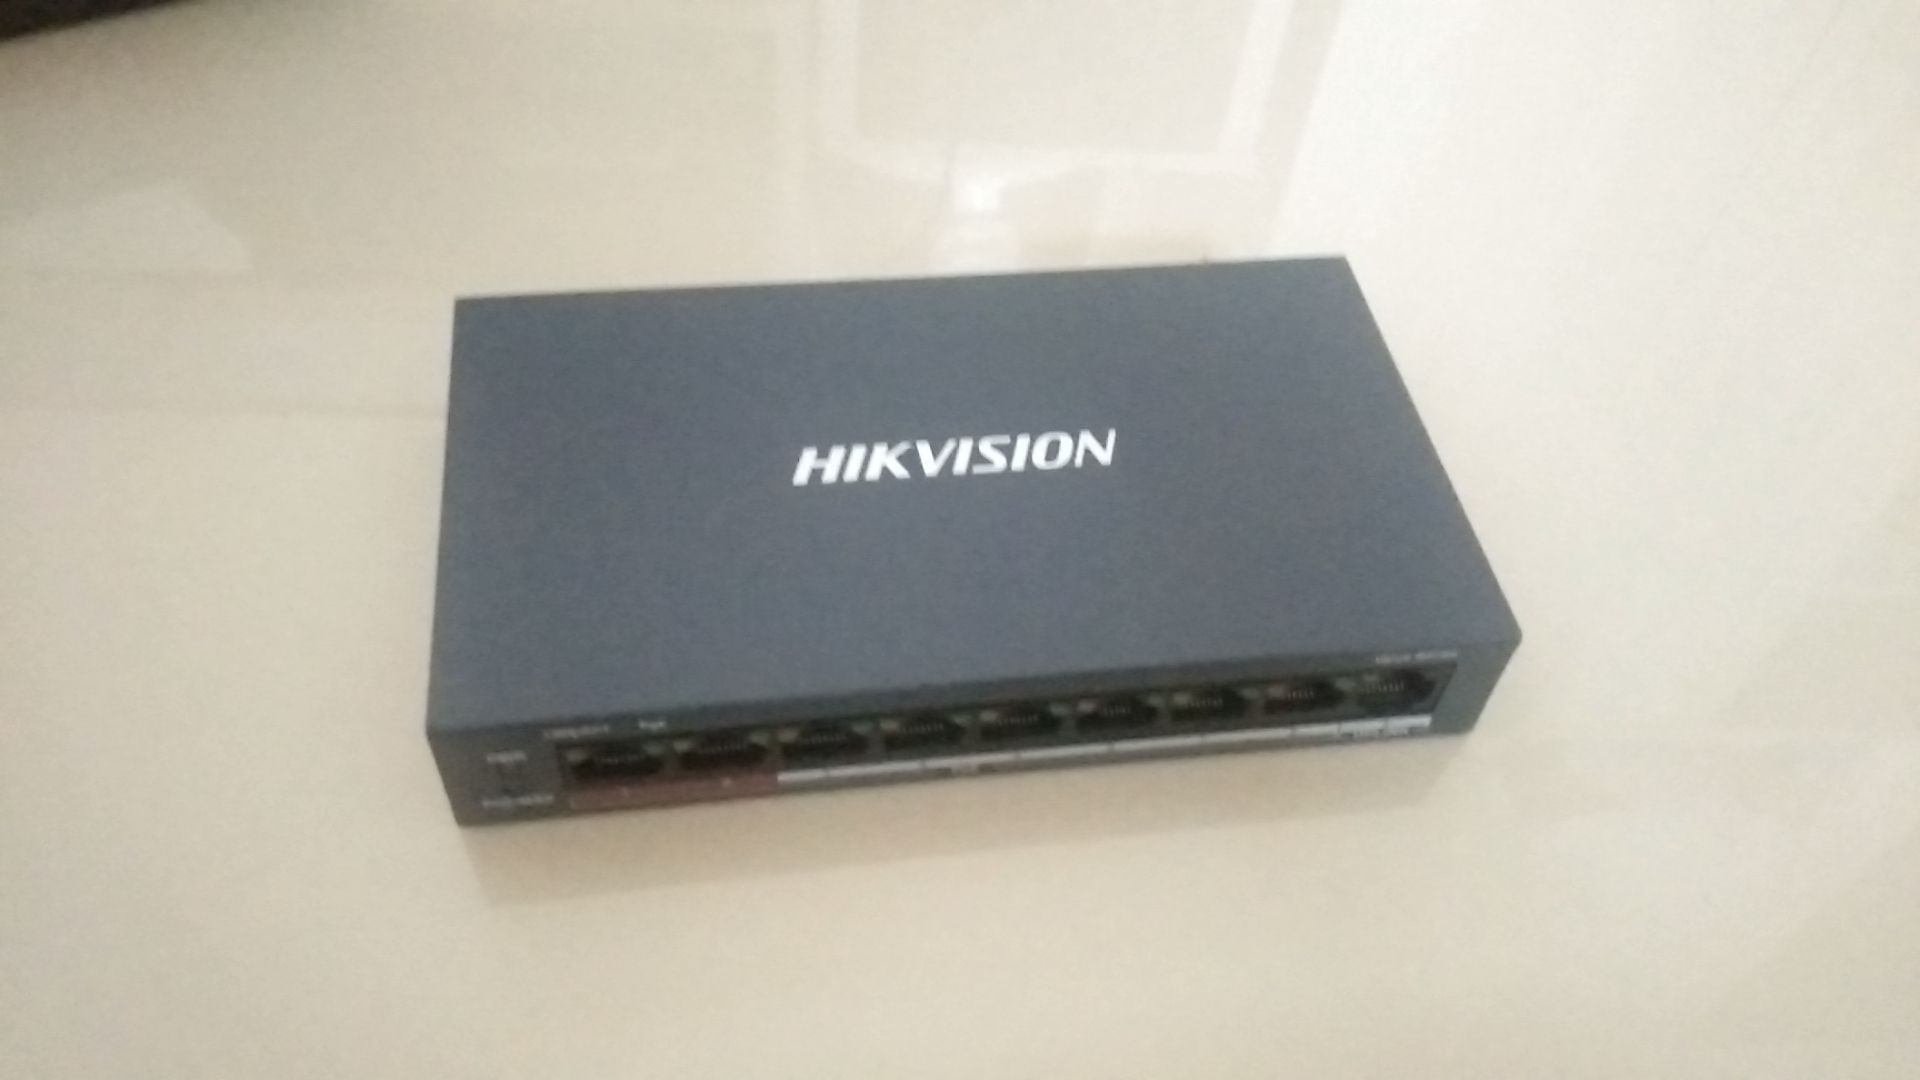
\includegraphics[scale=0.1]{gambar/cctvswitch.jpg}
  \caption{Switch}
  \label{fig:switch}

  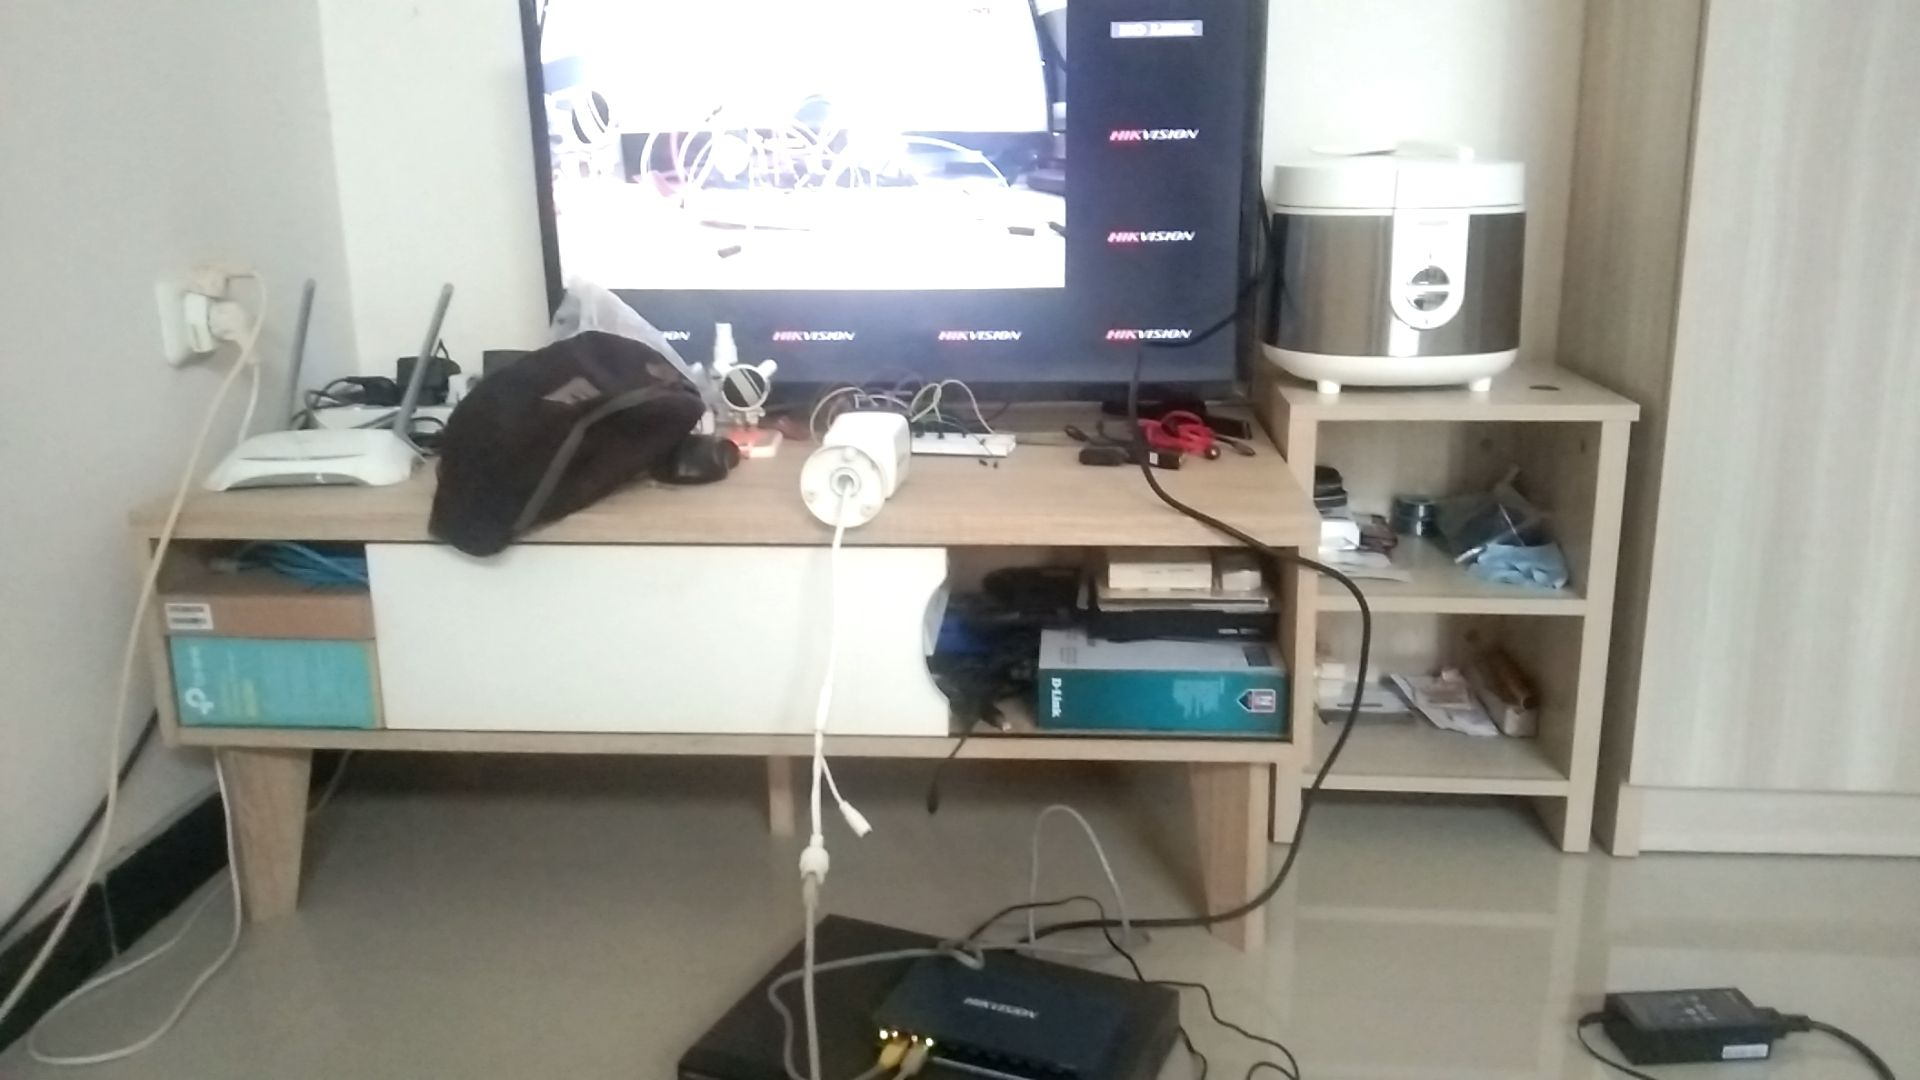
\includegraphics[scale=0.1]{gambar/cctvfullsistem.jpg}
  \caption{Full sistem CCTV yang telah terpasang}
  \label{fig:fullsistemcctv}
\end{figure}

% Contoh pembuatan code snippet
% \begin{lstlisting}[
%   language=C++,
%   label={lst:Hello World},
%   caption={Program hello world}
% ]
% #include <iostream>

% int main() {
%     std::cout << "Hello World!";
%     return 0;
% }
% \end{lstlisting}

% % Contoh penggunaan referensi dari code snippet yang diinputkan
% Seperti contoh pada baris program Listing \ref{lst:Hello World} dan Listing \ref{lst:PrimeNumber}, \lipsum[23]

% % Contoh input code snippet
% \lstinputlisting[
%   % Bahasa yang digunakan oleh code snippet
%   language=Python,
%   % Label referensi dari code snippet yang diinputkan
%   label={lst:PrimeNumber},
%   % Keterangan dari code snippet yang diinputkan
%   caption={Program perhitungan bilangan prima}
% % Nama dari file code snippet yang diinputkan
% ]{program/prime-number.py}

  \cleardoublepage

  % Bab 5 pengujian dan evaluasi
  % Ubah kalimat sesuai dengan judul dari bab ini
\chapter{PENGUJIAN DAN EVALUASI}

% Ubah konten-konten berikut sesuai dengan yang ingin diisi pada bab ini

\section{Skenario Pengujian}

Pengujian dilakukan dengan \lipsum[24]

\section{Evaluasi Pengujian}

Dari pengujian yang \lipsum[25][1-10]

% Contoh input konten dari file terpisah
% Contoh pembuatan tabel
\begin{longtable}{|l|l|l|}
  % Keterangan dari tabel yang dibuat
  \caption{Hasil Pengukuran Energi dan Kecepatan}
  % Label referensi dari tabel yang dibuat
  \label{tb:EnergiKecepatan}\\
  % Isi dari tabel yang dibuat
  \hline
  \rowcolor[HTML]{C0C0C0}
  \textbf{Energi} & \textbf{Jarak Tempuh} & \textbf{Kecepatan} \\ \hline
  10 J & 1000 M & 200 M/s \\ \hline
  20 J & 2000 M & 400 M/s \\ \hline
  30 J & 4000 M & 800 M/s \\ \hline
  40 J & 8000 M & 1600 M/s \\ \hline
\end{longtable}


% Contoh penggunaan referensi dari tabel yang dibuat
Sesuai dengan hasil pada Tabel \ref{tb:EnergiKecepatan}, didapatkan bahwa energi yang \lipsum[26]

  \cleardoublepage

  % Bab 6 kesimpulan dan saran
  % Ubah kalimat sesuai dengan judul dari bab ini
\chapter{KESIMPULAN DAN SARAN}

% Ubah konten-konten berikut sesuai dengan yang ingin diisi pada bab ini

\section{Kesimpulan}

Kesimpulan yang kami peroleh dari topik KP yang telah kami kerjakan ini adalah:

\begin{enumerate}[nolistsep]

  \item Siffars memiliki peforma pendeteksian dan pengenalan wajah yang baik namun juga diperlukan \texit{tunning} dan konfigurasi untuk mendapatkan performa tersebut

  \item Beberapa hal yang perlu diperhatikan untuk instalasi dan konfigurasi Siffars adalah, Setup GPU dan OpenCv yang diinstal menggunakan GPU support, Karena 2 hal tersebut sangat berpengaruh pada performa Siffars.

  \item Siffars memiliki beberapa versi, terdapat versi \texit{lite} yang lebih ringan daripada versi originalnya.

\end{enumerate}

\section{Saran}

Saran yang kami ajukan dalam pengerjaan KP ini antara lain:

\begin{enumerate}[nolistsep]

  \item Sistem deteksi wajah yang kami buat di \texit{web} menggunakan tensorflowJS sebagai \texit{engine}nya yang lebih berat daripada \texit{detector l}ain. Untuk versi ringannya dapat dicoba menggunakan \texit{tensorflowJS lite}.

  \item Input data foto yang digunakan dalam sistem Siffars menggunakan base64 \texit{encoding}, dimana lebih berat daripada menggunakan metode pengiriman gambar yang lain. Dapat dicoba menggunakan \texit{multipart-form} untuk mengirimkan gambar.

  \item Model deteksi wajah dari \texit{Siffars} menggunakan FaceNet sebagai basisnya. Dapat dicoba menggunakan model lain yang lebih ringan untuk mempercepat peforma dari Siffars.

\end{enumerate}

  \cleardoublepage

  % Daftar pustaka
  \renewcommand\bibname{DAFTAR PUSTAKA}
  \addcontentsline{toc}{chapter}{\bibname}
  \bibliographystyle{unsrtnat}
  \bibliography{pustaka/pustaka.bib}
  \cleardoublepage

  % Biografi penulis
  % \begin{center}
  \Large\textbf{BIOGRAFI PENULIS}
\end{center}
\vspace{2ex}

\addcontentsline{toc}{chapter}{BIOGRAFI PENULIS}

\begin{wrapfigure}{L}{0.3\textwidth}
  \centering
  \vspace{-3ex}
  % Ubah nama file gambar berikut dengan nama file foto dari mahasiswa pertama
  
\includegraphics[width=0.3\textwidth]{gambar/elon.jpg}
  \vspace{-4ex}
\end{wrapfigure}

% Ubah kalimat berikut dengan biografi dari mahasiswa pertama
\noindent Elon Reeve Musk, lahir pada \lipsum[1]

\vspace{2ex}

\begin{wrapfigure}{L}{0.3\textwidth}
  \centering
  \vspace{-3ex}
  % Ubah nama file gambar berikut dengan nama file foto dari mahasiswa kedua
  
\includegraphics[width=0.3\textwidth]{gambar/felix.jpg}
  \vspace{-4ex}
\end{wrapfigure}

% Ubah kalimat berikut dengan biografi dari mahasiswa kedua
\noindent Felix Arvid Ulf Kjellberg, lahir pada \lipsum[2]

  % \cleardoublepage

\end{document}
